% MDPI manuscript rebuilt around the narrowed corrupted-bearing story.
\documentclass[drones,article,submit,pdftex,moreauthors]{Definitions/mdpi}

\firstpage{1}
\makeatletter
\setcounter{page}{\@firstpage}
\makeatother
\pubvolume{1}
\issuenum{1}
\articlenumber{0}
\pubyear{2026}
\copyrightyear{2026}
\datereceived{}
\daterevised{}
\dateaccepted{}
\datepublished{}
\setlength{\headheight}{20pt}

\usepackage{amsmath}
\usepackage{booktabs}
\usepackage{tabularx}

\Title{Robust Front-End for Corrupted Bearing Fusion in Multi-UAV Passive Localization}

\Author{Zengye Su $^{1,*}$, Yudan Nie $^{1}$ and Zilu Zhou $^{2}$}
\AuthorNames{Zengye Su, Yudan Nie and Zilu Zhou}

\address{%
$^{1}$ \quad School of Information Technology and Engineering, Guangzhou College of Commerce, Guangzhou 511363, China; szy@xs.gcc.edu.cn (Z.S.); nyd@xs.gcc.edu.cn (Y.N.) \\
$^{2}$ \quad Guangzhou College of Commerce, Guangzhou 511363, China}

\corres{Correspondence: Zengye Su; szy@xs.gcc.edu.cn}

\abstract{This paper studies one-shot multi-UAV passive localization when a subset of bearing measurements is missing, biased, or grossly corrupted. The focus is the fusion front-end, while observer poses are supplied by an external navigation module with explicit pose uncertainty in evaluation. The proposed front-end combines consensus-style initialization, trimmed iteratively reweighted Gauss--Newton refinement, optional common-bias correction, and adaptive fixed-budget screening when only part of the bearing set can be fused. Across 2000 Monte Carlo cases, the median error decreases from 1.0792 to 0.1799 in the outlier regime and from 0.8547 to 0.3122 under mixed corruption. In 1844 PyBullet replay windows, the overall median error decreases from 4.4387 to 1.1539 and the catastrophic-failure rate decreases from 0.4675 to 0.1605. Threshold-sweep, tail-risk, and replay-tracking analyses show that the gain comes mainly from suppressing extreme failures rather than from small average-case changes. The method is therefore positioned as a reproducible robust fusion front-end for corrupted bearing sets in passive multi-UAV localization.}

\keyword{bearing-only localization; passive target localization; robust estimation; measurement screening; multi-UAV sensing; corrupted measurements}

\addhighlights{yes}
\renewcommand{\addhighlights}{%
\noindent\textbf{What are the main findings?}
\begin{itemize}[labelsep=2.5mm,topsep=-3pt]
\item A consensus-assisted robust fusion front-end sharply reduces catastrophic one-shot failures under outliers, mixed corruption, pose uncertainty, and heterogeneous bias.
\item Under fixed measurement budgets, geometry--reliability screening improves over residual-only, reliability-only, and geometry-only subset rules, while adaptive gating avoids unnecessary pruning.
\end{itemize}\vspace{3pt}
\textbf{What are the implications of the main findings?}
\begin{itemize}[labelsep=2.5mm,topsep=-3pt]
\item The contribution is an engineering front-end for passive multi-UAV localization, not a full autonomy stack, and it can be inserted between navigation/bearing extraction and downstream tracking or replanning.
\item Replay-based threshold, tail-risk, and downstream tracking-proxy results show that the main value lies in preventing unusable target cues rather than in marginally shifting average-case error.
\end{itemize}
}

\begin{document}

\section{Introduction}

Bearing-only passive sensing remains attractive for multi-UAV missions because it preserves low observability, reduces payload burden, and can still provide actionable target cues when active ranging or infrastructure support is unavailable \cite{avola2024uav,liu2025survey,kramaric2025comprehensive,gao2023scalable,li2025bearing}. In practice, however, the hardest failure mode is not lack of geometry alone. A one-shot localization cycle can fail because a few bearings are missing, heavily biased, grossly corrupted, or inconsistent with the rest of the set. Once those measurements enter the fusion step, the resulting position estimate may leave the local region in which it is still useful for downstream search, tracking, or handoff.

Recent UAV localization research has advanced quickly at the system level. Representative directions include tightly coupled integrated navigation, distributed cooperative localization, factor-graph or surveying-adjustment formulations, multi-condition constrained fusion, and learning-assisted cooperative inference \cite{yang2020tightly,dai2022uav,yang2024distributed,qian2025cooperative,li2025tcdrl,li2026formation,liu2026high,ding2026set,jia2024composite}. A second line of work focuses on bearing-only sensing itself, covering AOA-based formation positioning, path optimization, observability enhancement, CRLB-driven trajectory design, and passive node selection \cite{kang2024aoa,huang2025emcompat,xing2025node,zou2024revisit,chen2025variable,wang2025bio,dogancay2024bayesian}. These studies are valuable, but they do not directly solve the narrower question addressed here: given one fixed set of bearings in the current cycle, how should the estimator remain reliable when part of the set is corrupted?

That narrower question is not trivial. Recent work on error bounds, dynamic bearing processing, dual-UAV filtering, bearing-only circumnavigation, underwater passive localization, and distributed passive sensing all show that corrupted angular information can dominate localization quality \cite{chen2025error,luo2025dynamicbearing,yin2025dual,dou2025moving,mei2024bearing,zong2025distributed,yu2025passive,wu2026bearing,zhou2026direct,liu2026sensing}. Yet the response is often to change the path, redesign the observer geometry, or invoke a heavier cooperative back end. Those are important directions, but they leave a practical gap at the front end of the sensing pipeline: a mission system often needs a robust answer now, before a new trajectory or graph optimization can be recomputed.

From a UAV-systems perspective, that front-end gap is operationally meaningful. In practical passive sensing, bearings may be produced by gimballed electro-optical payloads, direction-finding antennas, or compact angle-only perception stacks whose outputs are constrained by field of view, asynchronous triggering, varying pose quality, and limited uplink budget \cite{chen2025research,peng2024trajectory,zhou2026target,zhang2026multi}. A planner or downstream tracker cannot benefit from those measurements if the localization front end collapses as soon as a few bearings become unreliable. This motivates a narrower but still UAV-relevant question: how much robustness can be recovered inside one sensing cycle before invoking a heavier back end?

The second motivation is methodological. A large fraction of the localization literature either emphasizes geometry optimization or assumes a sequential estimator that can smooth errors over time. Those directions are important, but they do not remove the need for a robust one-shot estimate when a mission stack must react immediately. Moreover, sim-to-real studies in UAV autonomy repeatedly show that apparently small disturbances in attitude, delay, and synchronization can produce large downstream degradation if the front end is brittle \cite{panerati2021learning,perezsegui2023bridging}. For this reason, the present manuscript expands the validation chain beyond static Monte Carlo to include pseudo-physical replay and a multi-vehicle PyBullet replay layer.

This paper studies one-shot planar multi-observer bearing-only localization under corrupted measurements. The target is the fusion front-end inside a passive sensing stack: a robust estimator suppresses failures caused by bad bearings, and an optional screening stage is activated when only a limited number of measurements can be fused or transmitted. This scope matches the evidence provided by the experiments and the intended engineering use of the method.

This problem definition leads to three concrete design requirements. First, the front end must remain numerically stable when only a minority of bearings are unreliable, because a tactical UAV system often has to act before a new trajectory or full graph optimization is available. Second, the method should degrade gracefully when a bandwidth or compute budget forces the system to retain only part of the current bearing set; this motivates treating screening as a conditional budget-management module rather than as a universal replacement for full-set fusion. Third, the evidence should move beyond static geometry, because in practice the usefulness of a one-shot cue is determined by whether it remains consumable after timing variation, attitude disturbance, and navigation error are introduced. The architecture and validation chain used in the rest of the paper follow these three requirements directly.

The main contributions are threefold:
\begin{itemize}
\item a consensus-assisted robust bearing-only estimator that combines multi-start geometric initialization, trimmed iteratively reweighted refinement, optional common-bias correction, and a consensus fallback;
\item a reliability-adaptive screening module for fixed-budget settings, together with residual-only, reliability-only, geometry-only, and adaptive baselines that clarify when screening is useful and when all-sensor robust fusion should be kept;
\item a reproducible validation chain comprising 2000 Monte Carlo cases across five corrupted-measurement regimes, a 1716-case fixed-budget screening benchmark, pseudo-physical dynamic replay with delay, jitter, per-sensor bias, and motion-induced disturbance, and a 1844-case PyBullet multi-vehicle replay study.
\end{itemize}

The remainder of the paper is organized as follows. Section~2 reviews related work. Section~3 formulates the corrupted-measurement localization problem. Section~4 presents the proposed estimation and screening framework. Section~5 describes the experimental protocol, Section~6 reports the results, and Sections~7 and~8 discuss the scope and conclude the paper.

\section{Related Work}

\subsection{Bearing-Only and Passive Localization}

Bearing-only and passive target localization remain active topics in UAV and distributed sensing research because they support low-emission observation and can be combined with cooperative formations \cite{li2025bearing,kang2024aoa,huang2025emcompat,xing2025node}. Recent studies investigate D-criterion and Bayesian-FIM trajectory planning \cite{zou2024revisit,dogancay2024bayesian}, CRLB-based variable-speed path design \cite{chen2025variable,peng2024trajectory}, observability enhancement with sensor-bias estimation \cite{wang2025bio}, and bearing-only control with experimental disturbance handling \cite{sui2024adaptive,dou2025moving}. Related developments also appear in underwater passive localization, wideband array localization, direct target localization, and passive source localization in other sensing domains \cite{mei2024bearing,zong2025distributed,yu2025passive,wu2026bearing,zeng2026three,zhou2026direct,chen2025research}. The common thread is that geometry matters, but corrupted or uncertain bearings can still dominate the final error.

\subsection{Robust Estimation Under Corrupted Angular Measurements}

The literature increasingly recognizes that bearing quality is heterogeneous. Error-bound studies, dynamic bearing-angle analysis, multi-array likelihood processing, and dual-UAV filtering all show that uncertainty handling is at least as important as nominal geometry under realistic disturbances \cite{chen2025error,luo2025dynamicbearing,hu2025cyclic,yin2025dual}. Classical least squares is usually too fragile in the presence of outliers, observer-pose uncertainty, or mixed corruption, while generic stochastic search methods are often computationally heavy or hard to interpret. Standard robust choices such as Huber, Tukey, consensus-style filtering, or particle-based inference are therefore natural baselines, but they are rarely packaged as an explicit front-end block for fixed corrupted bearing sets in multi-UAV passive sensing. In particular, recent UAV papers still devote more attention to trajectory or formation design than to the behavior of the current-cycle estimator when a few bearings become severely unreliable \cite{li2025bearing,huang2025emcompat,zhou2026target}.

\subsection{Sensor Selection, Observability, and Budgeted Sensing}

The second topic relevant to this paper is sensing selection. Passive node selection, observability-aware planning, and FIM/CRLB-based trajectory design are well established in the broader literature \cite{xing2025node,chen2025variable,wang2025bio,zou2024revisit,genadot2025about}. At the system level, collaborative UAV localization has also advanced through factor graphs, distributed inference, relative localization, and swarm-level cooperative frameworks \cite{yang2020tightly,yang2024distributed,qian2025cooperative,li2025tcdrl,li2026formation,ding2026set,zhang2026multi}. The present work is narrower than those frameworks. It addresses a centralized one-shot decision: once a set of bearings has already been produced for the current cycle, should all of them be fused, or should a smaller subset be retained because the current quality is too uneven? That framing is closer to front-end measurement triage than to long-horizon planning.

\subsection{Validation Gap and Manuscript Positioning}

Another gap is validation style. Public UAV-systems papers are increasingly expected to move beyond idealized static geometry and toward simulation pipelines that reflect timing, attitude, and coordination effects \cite{panerati2021learning,perezsegui2023bridging}. This is especially true for Drones-oriented work, where the distinction between a generic localization algorithm and a UAV-facing sensing paper often depends on whether the validation includes multi-vehicle trajectories, communication limits, or deployment-shaped disturbances. The present manuscript still stops short of hardware-in-the-loop or field tests, but it attempts to close part of that gap through pseudo-physical replay and PyBullet multi-vehicle replay. Appendix~A positions the manuscript explicitly against nearby representative studies, clarifying that the current contribution is a corrupted-bearing front end rather than a full collaborative autonomy stack.

\section{Problem Formulation}

We consider one localization cycle with $N$ observing platforms. The true planar observer positions are denoted by
\begin{equation}
\bar{s}_i = [\bar{x}_i,\bar{y}_i]^T,\qquad i=1,\dots,N,
\end{equation}
and the target position is
\begin{equation}
p = [x,y]^T.
\end{equation}
The estimator does not assume access to a full navigation stack. Instead, it receives reported observer poses
\begin{equation}
s_i = \bar{s}_i + n_{s,i},
\end{equation}
where $n_{s,i}$ models pose error from an external navigation module such as VIO, INS, or SLAM. This assumption resolves the usual tension between GNSS-denied mission language and known observer poses: the present paper studies the bearing-fusion block, not the upstream self-localization module.

Each valid observer contributes one bearing measurement:
\begin{equation}
\theta_i = \operatorname{atan2}(y-\bar{y}_i, x-\bar{x}_i) + b_c + b_i + \epsilon_i + o_i,
\end{equation}
where $b_c$ is a shared frame-level bias, $b_i$ is a sensor-specific bias, $\epsilon_i$ is nominal noise, and $o_i$ represents occasional gross corruption. A measurement may also be missing because of detection failure, occlusion, or communication loss. For a candidate target position $p$, the predicted bearing uses the reported pose:
\begin{equation}
\hat{\theta}_i(p;s_i)=\operatorname{atan2}(y-y_i,x-x_i).
\end{equation}
The wrapped residual is
\begin{equation}
r_i(p,b_c)=\operatorname{wrap}\!\left(\hat{\theta}_i(p;s_i)-\theta_i-b_c\right),
\end{equation}
where $\operatorname{wrap}(\cdot)$ maps an angle to $(-\pi,\pi]$.

The paper studies a one-shot planar setting with three explicit scope boundaries. First, the estimator is centralized and uses the current cycle only; it is not a sequential tracker or a distributed fusion protocol. Second, the reported observer poses are treated as inputs, but pose uncertainty is injected into the benchmark. Third, the geometry is planar; the paper targets fixed-height or small-height-difference settings and leaves full three-dimensional extension to future work.

The experimental thresholds are normalized by the formation radius $R$. In the main Monte Carlo benchmark, $R=10$, so success at $0.1R$ corresponds to absolute error $\leq 1.0$, and catastrophic failure at $0.5R$ corresponds to absolute error $>5.0$. These thresholds are intended to distinguish locally usable cues from clearly misleading ones.

\subsection{Operational Constraint Model}

The manuscript treats measurement screening as an engineering response to limited fusion budget rather than as a universal replacement for all-sensor estimation. Let $z_i\in\{0,1\}$ indicate whether bearing $i$ is transmitted or fused. Then the budgeted front-end problem is
\begin{equation}
\sum_{i=1}^{N} z_i \leq k,\qquad 3 \leq k < N,
\end{equation}
where $k$ reflects a fixed communication, computation, or timing budget for the current cycle. In practice, this budget corresponds to cases such as delayed uplink from a subset of vehicles, reduced onboard processing time, or a front-end module that is allowed to keep only a limited number of bearings before passing a candidate target cue downstream. The baseline against which screening should be judged is therefore not ``all-sensor robust fusion is always worse'', but rather ``when a subset must be used, can the subset be chosen more intelligently than with naive rules?''.

\subsection{Corruption Taxonomy and Applicability}

The expanded benchmark distinguishes four practically important error sources. First, \emph{outliers} model gross bearing corruption produced by spurious detections, local clutter, or momentary payload faults. Second, \emph{missing observations} model occlusion, field-of-view truncation, or communication dropouts. Third, \emph{shared or heterogeneous bias} models heading-reference mismatch, platform-frame misalignment, or per-sensor directional bias. Fourth, \emph{observer-pose uncertainty} represents the fact that the bearing-fusion module depends on an upstream navigation subsystem whose errors propagate into the current localization cycle. These are still abstractions, but they map more cleanly to the UAV sensing stack than a single isotropic-noise assumption.

Figure~\ref{fig:systempipeline} shows the system boundary used throughout the paper. Observer poses and angle cues enter the corruption-aware front end, which returns a one-shot target cue and confidence estimate to downstream tracking, handoff, or replanning modules.

\begin{figure}[!htbp]
\centering

\includegraphics[width=0.98\linewidth]{../figures/figure_system_pipeline}
\caption{Operational position of the proposed method in a passive multi-UAV sensing stack. The paper focuses on the corruption-aware front end between upstream self-localization and bearing extraction modules and downstream tracking, handoff, or replanning modules.}
\label{fig:systempipeline}
\end{figure}

\subsection{Application Scenarios and User Pain Points}

Three application scenarios motivate the current scope. The first is electromagnetically silent or low-emission cooperative observation, where several UAVs observe a noncooperative target without active ranging \cite{li2025bearing,huang2025emcompat}. In this setting, the operator's pain point is not only global observability. The immediate problem is that a small number of bad bearings can move the fused cue far enough that a downstream confirmation camera or interceptor will search the wrong neighborhood. A front end that suppresses those large one-shot failures is therefore valuable even before one discusses long-horizon formation control.

The second scenario is communication-limited swarm cueing. In many practical stacks, not every vehicle can upload every measurement at full rate, especially when edge compute, bandwidth, or synchronization budget is limited. This is the use case behind the optional screening module. The question is not whether subset selection is universally superior to all-sensor fusion. The question is whether, once a subset must be retained, the system can avoid obviously poor triage decisions. Framed this way, the measurement-screening module addresses a concrete engineering bottleneck rather than an abstract optimization game.

The third scenario is degraded navigation and asynchronous payload operation. Passive bearings are often produced by vision, gimbal, or direction-finding modules whose timestamps, headings, and internal quality are not perfectly aligned. At the same time, the observer poses delivered by GNSS, VIO, INS, or SLAM are themselves imperfect. This coupling between pose uncertainty and bearing corruption is precisely where contest-style least squares tends to become brittle. The present paper therefore focuses on the narrow but operationally meaningful question of what can be recovered inside one cycle before a tracker, planner, or human operator receives the cue.

\begin{table}[!htbp]
\centering
\caption{Representative passive-sensing deployment scenarios and their dominant corruption sources.}
\label{tab:deploymain}
\small
\begin{tabularx}{\linewidth}{>{\RaggedRight\arraybackslash}p{0.23\linewidth} >{\RaggedRight\arraybackslash}p{0.23\linewidth} X}
\toprule
Scenario & Dominant corruption sources & Why the present front end is relevant \\
\midrule
Electromagnetically silent formation sensing \cite{li2025bearing,huang2025emcompat} & Shared heading bias, geometry imbalance, communication-limited updates & A robust one-shot fusion block suppresses catastrophic cue displacement before formation redesign or long-horizon planning is invoked. \\
Communication-limited swarm cueing \cite{xing2025node,zhou2026target} & Uneven node quality, delayed uplink, bandwidth budget & The fixed-budget screening module is explicitly motivated by this regime and is evaluated against residual-only, reliability-only, and geometry-only subset rules. \\
Degraded navigation and asynchronous payload operation \cite{chen2025research,peng2024trajectory} & Pose error, timestamp mismatch, intermittent detections, bearing drift & The pose-uncertainty, heterogeneous-bias, pseudo-physical replay, and PyBullet replay layers target this failure pattern directly. \\
Simulation-to-real transition studies \cite{panerati2021learning,perezsegui2023bridging} & Delay, attitude disturbance, bias drift, replay mismatch & The manuscript positions the method as an intermediate front-end baseline that should later be coupled to SITL, HITL, or field-log replay. \\
\bottomrule
\end{tabularx}
\end{table}


Table~\ref{tab:deploymain} summarizes why the current corruption taxonomy is not merely an abstract noise menu. Each scenario maps to a concrete systems question that appears in passive UAV sensing: whether a cue remains usable under heading bias, whether limited uplink bandwidth should trigger subset triage, whether asynchronous payloads and pose drift destabilize the current estimate, and whether a simulation-only study is at least moving toward a more realistic validation chain. Making these correspondences explicit helps keep the manuscript focused on a front-end sensing problem with operational consequences rather than on a generic optimization exercise.

\section{Materials and Methods}

\subsection{Framework Overview}

The proposed framework has two stages. Stage~1 is a robust localization core. It receives all currently valid bearings, generates several candidate target hypotheses, refines them under trimmed iteratively reweighted estimation, and keeps the hypothesis with the smallest final residual. Stage~2 is optional. When only a limited number of bearings can be fused or transmitted, it screens the current set using geometry and residual reliability. An adaptive gate bypasses screening and keeps all-sensor robust fusion when the current bearing set looks sufficiently homogeneous.

This decomposition treats localization as an engineering front-end problem. The estimator sits between navigation/bearing extraction modules and downstream planning or tracking modules, and it is designed to remain lightweight enough for repeated use within the current sensing cycle.

\subsection{Consensus-Assisted Robust Estimation}

\paragraph{Geometric candidate generation.}
For observer $i$, the bearing ray is
\begin{equation}
\ell_i(\tau_i)=s_i+\tau_i
\begin{bmatrix}
\cos\theta_i\\
\sin\theta_i
\end{bmatrix}.
\end{equation}
Pairwise ray intersections generate an initial candidate pool. The implementation keeps several consensus-style representatives of that pool, including the centroid, the coordinate-wise median, and a trimmed centroid. In addition, a consensus hypothesis is obtained by a RANSAC-style pass so that heavily contaminated cases have an explicit fallback hypothesis before iterative refinement begins.

\paragraph{Robust objective and Jacobian.}
For active measurements, the estimator minimizes
\begin{equation}
\min_{p,b_c}\sum_{i=1}^{N} w_i\,\rho\!\left(r_i(p,b_c)\right),
\end{equation}
where $\rho(\cdot)$ is implemented through iteratively reweighted least squares and the weights are updated after trimming large residuals. Let
\begin{equation}
d_i^2=(x-x_i)^2+(y-y_i)^2.
\end{equation}
The bearing Jacobian with respect to the target position is
\begin{equation}
\mathbf{J}_i(p)=
\begin{bmatrix}
-\dfrac{y-y_i}{d_i^2} &
\dfrac{x-x_i}{d_i^2}
\end{bmatrix}.
\end{equation}
The code uses a damped Gauss--Newton/Levenberg--Marquardt step rather than finite-difference gradient descent. With $A_i=[\mathbf{J}_i\;\;-1]$ when common-bias correction is active, the linearized update solves
\begin{equation}
\Delta = -\left(A^TWA+\lambda I\right)^{-1}A^TWr,
\end{equation}
where $W$ is the diagonal matrix of current robust weights and $\lambda$ is a small damping term.

\paragraph{Trimmed iteratively reweighted refinement.}
The robust core updates weights from the residual pattern, trims the largest residuals, and then refines the estimate by several damped Gauss--Newton steps. Tukey-type downweighting is used after trimming so that the tail of the residual distribution is suppressed more aggressively than in plain Huber IRLS. The common-bias term is updated only when the active residuals are sufficiently concentrated; otherwise the algorithm falls back to zero bias rather than forcing an unstable common correction onto heterogeneous measurements. After refinement, a consensus fallback is retained when the residual tail remains too heavy. In this sense, the proposed estimator is not a single trick but a small robust front-end that combines geometric hypotheses, trimming, reweighting, and consensus rescue.

\paragraph{Algorithmic summary.}
The robust estimator can be summarized as follows. First, generate a pool of pairwise-intersection hypotheses together with consensus-style summary points. Second, evaluate a RANSAC-like fallback hypothesis so that a heavily corrupted case still has a viable initial anchor. Third, refine each candidate by several rounds of trimmed reweighting and damped Gauss--Newton updates, optionally correcting a shared bias when the active residuals are concentrated enough. Fourth, retain the candidate with the lowest final robust residual. Fifth, if the residual tail after refinement remains too heavy, fall back to the best consensus hypothesis. This sequence is intentionally simple enough to reproduce from the codebase while still addressing the main failure modes seen in corrupted bearing sets.

\subsection{Reliability-Adaptive Measurement Screening}

The screening stage starts from the pilot estimate delivered by Stage~1. Residual reliability is computed from the current residuals, and screening is invoked only in fixed-budget settings or when the adaptive gate considers the current residual pattern too heterogeneous to trust all measurements equally.

For a candidate subset $\mathcal{S}$, the weighted geometry matrix is
\begin{equation}
\mathbf{F}_{\mathcal{S}}=\sum_{i\in\mathcal{S}} w_i\,\mathbf{J}_i^T\mathbf{J}_i,
\end{equation}
and the isotropy term is
\begin{equation}
\eta_{\mathcal{S}}=\frac{\lambda_{\min}(\mathbf{F}_{\mathcal{S}})}{\lambda_{\max}(\mathbf{F}_{\mathcal{S}})}.
\end{equation}
The proposed normalized screening score is
\begin{equation}
\operatorname{Score}(\mathcal{S})=
0.34\,\phi_{\det}(\mathcal{S})
+0.18\,\eta_{\mathcal{S}}
+0.24\,\bar{w}_{\mathcal{S}}
+0.24\,\phi_{r}(\mathcal{S}),
\end{equation}
where
\begin{equation}
\phi_{\det}(\mathcal{S}) = 1-\exp\!\left(-10^4\det(\mathbf{F}_{\mathcal{S}})\right),
\qquad
\phi_r(\mathcal{S}) = 1-\min\!\left(\frac{\bar{r}_{\mathcal{S}}}{0.25},1\right),
\end{equation}
and $\bar{w}_{\mathcal{S}}$ and $\bar{r}_{\mathcal{S}}$ denote the mean reliability and mean absolute residual on the subset. The score uses four normalized ingredients and avoids stacking several strongly correlated geometry terms.

The score should be read as a tractable surrogate for a small budgeted search problem rather than as a universal law. In idealized form, the screening objective can be expressed as
\begin{equation}
\mathcal{S}^{\star}=
\arg\max_{|\mathcal{S}|=k}
\Big[
\alpha_1 \phi_{\det}(\mathcal{S})
+\alpha_2 \eta_{\mathcal{S}}
+\alpha_3 \bar{w}_{\mathcal{S}}
+\alpha_4 \phi_r(\mathcal{S})
\Big],
\end{equation}
with fixed coefficients $\alpha_1,\dots,\alpha_4$ chosen once and then held constant across the reported experiments. The implementation evaluates this objective over a capped reliability-sorted pool so that the search remains computationally small.

The proposed policy performs a small exhaustive search over a top-reliability candidate pool, which is feasible because the pool is capped in the experiments. Baselines include random subset selection, angular-spread greedy selection, FIM-only greedy selection, residual-only top-$k$, reliability-only top-$k$, and the all-sensor robust estimator. The adaptive policy uses all-sensor robust fusion when the residual median absolute deviation and reliability dispersion are both small; otherwise it activates screening. This makes screening a conditional tool rather than a default law. Because a reviewer can reasonably ask whether the chosen coefficient vector is too brittle, Section~6 revisits the screening score under explicit coefficient perturbations rather than only reporting a single frozen setting.

\subsection{Complexity and Reproducibility}

The geometric candidate generation stage is $O(N^2)$ because it depends on pairwise intersections. Each inner Gauss--Newton update is linear in the number of active measurements, while the number of outer reweighting rounds is fixed by configuration. In the screening stage, the exhaustive search is confined to a small top-reliability pool, so the practical cost is bounded by $\binom{m}{k}$ with small $m$ rather than by exhaustive search over the full sensor set. All experiments reuse the same Python package interfaces, and all manuscript figures are generated from frozen JSON outputs rather than from manually edited spreadsheets.

\subsection{Implementation Details and Default Settings}

The implementation uses a trim ratio of 0.15, three outer reweighting rounds, Huber scale 0.08, Tukey cutoff 0.18, and LM damping $10^{-3}$ as default settings. The adaptive gate keeps all-sensor fusion when the residual median absolute deviation is below 0.05 and the reliability dispersion is below 0.12. The fixed-budget screening benchmark sets the budget to approximately 55\% of currently valid bearings, while the exhaustive search is confined to a capped top-reliability pool. These settings are not retuned from regime to regime; they are fixed across the expanded experimental matrix. Appendix~B lists the exact values together with their engineering interpretation and the experiments in which they were stress-tested.

\section{Experimental Protocol}

\subsection{Main Monte Carlo Benchmark}

The main synthetic benchmark contains 2000 cases. Five corrupted-measurement regimes are evaluated: clean, outlier, mixed, pose uncertainty, and heterogeneous bias. Each regime is run over 200 random seeds and two formations (circular and random) with eight observers. The formation radius is fixed at $R=10$, the target is placed at $(2.5,-1.5)$, and one bearing is generated per valid observer. The outlier regime uses outlier rate $0.28$ and scale $0.42$. The mixed regime combines common bias $0.04$, missing rate $0.20$, outlier rate $0.22$, and outlier scale $0.45$. The pose-uncertainty regime injects observer-pose noise of standard deviation $0.35$. The heterogeneous-bias regime uses sensor-specific bias standard deviation $0.05$ in addition to a small common bias.

The baseline estimators are nonlinear least squares, Huber IRLS, GNC with a Geman--McClure robustifier, and RANSAC. The proposed method is evaluated under the same interface and with the same reported observer poses. The main metrics are median error, mean error, 90th-percentile error, success at $0.1R$, and catastrophic failure above $0.5R$. Bootstrap 95\% confidence intervals are reported for the medians.

\subsection{Fixed-Budget Screening Benchmark}

The screening benchmark contains 1716 cases over mixed and severe regimes, three formation families (circle, perturbed, and random), and 8/10/12-observer settings. The subset budget is approximately 55\% of the currently valid measurements, clipped to remain strictly smaller than the full set. This benchmark is designed to answer a narrower question than the main estimator benchmark: not whether screening beats unconstrained all-sensor robust fusion, but whether a budgeted policy can use the limited subset more effectively than simple residual-only, reliability-only, geometry-only, or random screening.

\subsection{Pseudo-Physical Dynamic Replay}

To narrow the gap between static geometry and UAV-like dynamics, a pseudo-physical replay benchmark is also included. The replay generator injects motion-dependent delay, per-sensor bias, attitude-jitter-like disturbance, missing observations, and outliers before the current fusion cycle is evaluated. Forty seeds, three formations, and three swarm sizes produce 720 dynamic cases over mild and harsh regimes. This layer remains simulation-based, but it is closer to flight-like corruption than a purely static Monte Carlo sweep.

\subsection{PyBullet Multi-Vehicle Replay}

To further reduce the gap between static geometry and UAV-like temporal disturbance, we also replay bearing measurements from a multi-vehicle PyBullet environment derived from the \texttt{gym-pybullet-drones} ecosystem \cite{panerati2021learning}. The replay uses circle and ellipse formations with 8 and 10 vehicles, warm-up phases, time-sampled trajectories, gust-like disturbance, attitude-induced bearing perturbation, delay-step variation, missing observations, and slowly drifting common bias. The resulting benchmark contains 1844 replayed localization cycles over nominal and disturbed regimes. Although the current study still does not reach hardware-in-the-loop, this replay layer follows the broader UAV-validation recommendation that algorithm papers should test against timing and disturbance sources that are closer to actual vehicle dynamics \cite{perezsegui2023bridging}.

\subsection{Additional Generalization and Efficiency Analyses}

Beyond the headline benchmarks, the manuscript includes five auxiliary analyses. First, a formation-generalization study compares circular, elliptical, perturbed, and random observer layouts under mixed corruption. Second, sensor-count scaling evaluates 4/6/8/10/12-observer settings for both circle and random formations. Third, sensitivity sweeps vary outlier rate, common bias magnitude, and nominal noise level. Fourth, ablation, observability, and runtime studies isolate the effect of trimming, bias estimation, reweighting, geometry quality, and computational burden. Fifth, a screening-weight sensitivity study evaluates the exact $0.8\times/1.0\times/1.2\times$ grid for the four normalized screening coefficients on the same 432-window slice used for the earlier randomized stress test. These analyses do not replace the main benchmark, but they are important for showing where the method is fragile, where it generalizes, and what computational price is paid for the robustness gains.

\section{Results}

\subsection{Robust Localization Under Corrupted Bearings}

Table~\ref{tab:mainregimes} and Figure~\ref{fig:storyregimes} report the main result: corrupted measurements cause clear failures for least squares, while robust front-end estimation materially reduces both median error and failure risk. In the outlier regime, the median error decreases from 1.0792 for least squares to 0.1799 for the proposed method. In the mixed regime, it decreases from 0.8547 to 0.3122. These are not marginal differences: they represent a shift from brittle one-shot localization to a front-end that stays usable after bad bearings enter the set.

\begin{table}[!htbp]
\centering
\caption{Median localization error across the main corrupted-measurement regimes. Results aggregate 2000 Monte Carlo cases over clean, outlier, mixed, pose-uncertainty, and heterogeneous-bias settings with circular and random formations.}
\label{tab:mainregimes}
\begin{tabular}{lrrrrr}
\toprule
Regime & LS & Huber & GNC-GM & RANSAC & Proposed \\
\midrule
Clean                & 0.1052 & 0.1052 & 0.1043 & 0.1052 & 0.1052 \\
Outlier              & 1.0792 & 0.3458 & 0.3542 & 0.1792 & 0.1799 \\
Mixed                & 0.8547 & 0.4072 & 0.4167 & 0.3123 & 0.3122 \\
Pose Uncertainty     & 0.5739 & 0.3667 & 0.3702 & 0.3522 & 0.3513 \\
Heterogeneous Bias   & 0.4224 & 0.3533 & 0.3602 & 0.3323 & 0.3254 \\
\bottomrule
\end{tabular}
\end{table}

\begin{table}[!htbp]
\centering
\caption{Detailed statistics in the two hardest synthetic regimes. Thresholds are normalized by the formation radius $R=10$: success at $0.1R$ and catastrophic failure above $0.5R$.}
\label{tab:hardregimes}
\small
\begin{tabular}{llrrr}
\toprule
Regime & Method & Median [95\% CI] & Success@0.1R & Cat.@0.5R \\
\midrule
Outlier & Least Squares & 1.0792 [0.8748, 1.1428] & 0.4875 & 0.0025 \\
Outlier & GNC-GM        & 0.3542 [0.3147, 0.3870] & 0.8625 & 0.0025 \\
Outlier & RANSAC        & 0.1792 [0.1579, 0.2036] & 0.9375 & 0.0100 \\
Outlier & Proposed      & 0.1799 [0.1585, 0.2041] & 0.9400 & 0.0100 \\
\midrule
Mixed   & Least Squares & 0.8547 [0.7733, 0.9437] & 0.5625 & 0.0125 \\
Mixed   & GNC-GM        & 0.4167 [0.3479, 0.4707] & 0.8150 & 0.0200 \\
Mixed   & RANSAC        & 0.3123 [0.2905, 0.3442] & 0.8925 & 0.0175 \\
Mixed   & Proposed      & 0.3122 [0.2913, 0.3423] & 0.8925 & 0.0175 \\
\bottomrule
\end{tabular}
\end{table}


The comparison against stronger robust baselines is also informative. Huber IRLS and GNC-GM are both much better than least squares, but they remain consistently behind the proposed front end in the mixed, pose-uncertainty, and heterogeneous-bias regimes. RANSAC is a strong baseline in outlier-dominated settings, and the proposed method essentially matches it there while remaining slightly better in the mixed, pose-uncertainty, and heterogeneous-bias settings. This pattern is consistent with the design of the method: consensus helps under gross corruption, but trimmed reweighting and bias handling matter once the corruption is more heterogeneous.

The pose-uncertainty and heterogeneous-bias results are particularly important for the scope of the paper. They show that the revised benchmark is no longer built around ideal observer poses and shared-noise assumptions only. Under pose uncertainty, the median error decreases from 0.5739 for least squares to 0.3513 for the proposed method. Under heterogeneous bias, it decreases from 0.4224 to 0.3254. These improvements are smaller than in the outlier regime, but they address more realistic failure modes for practical passive sensing.

\begin{figure}[!htbp]
\centering
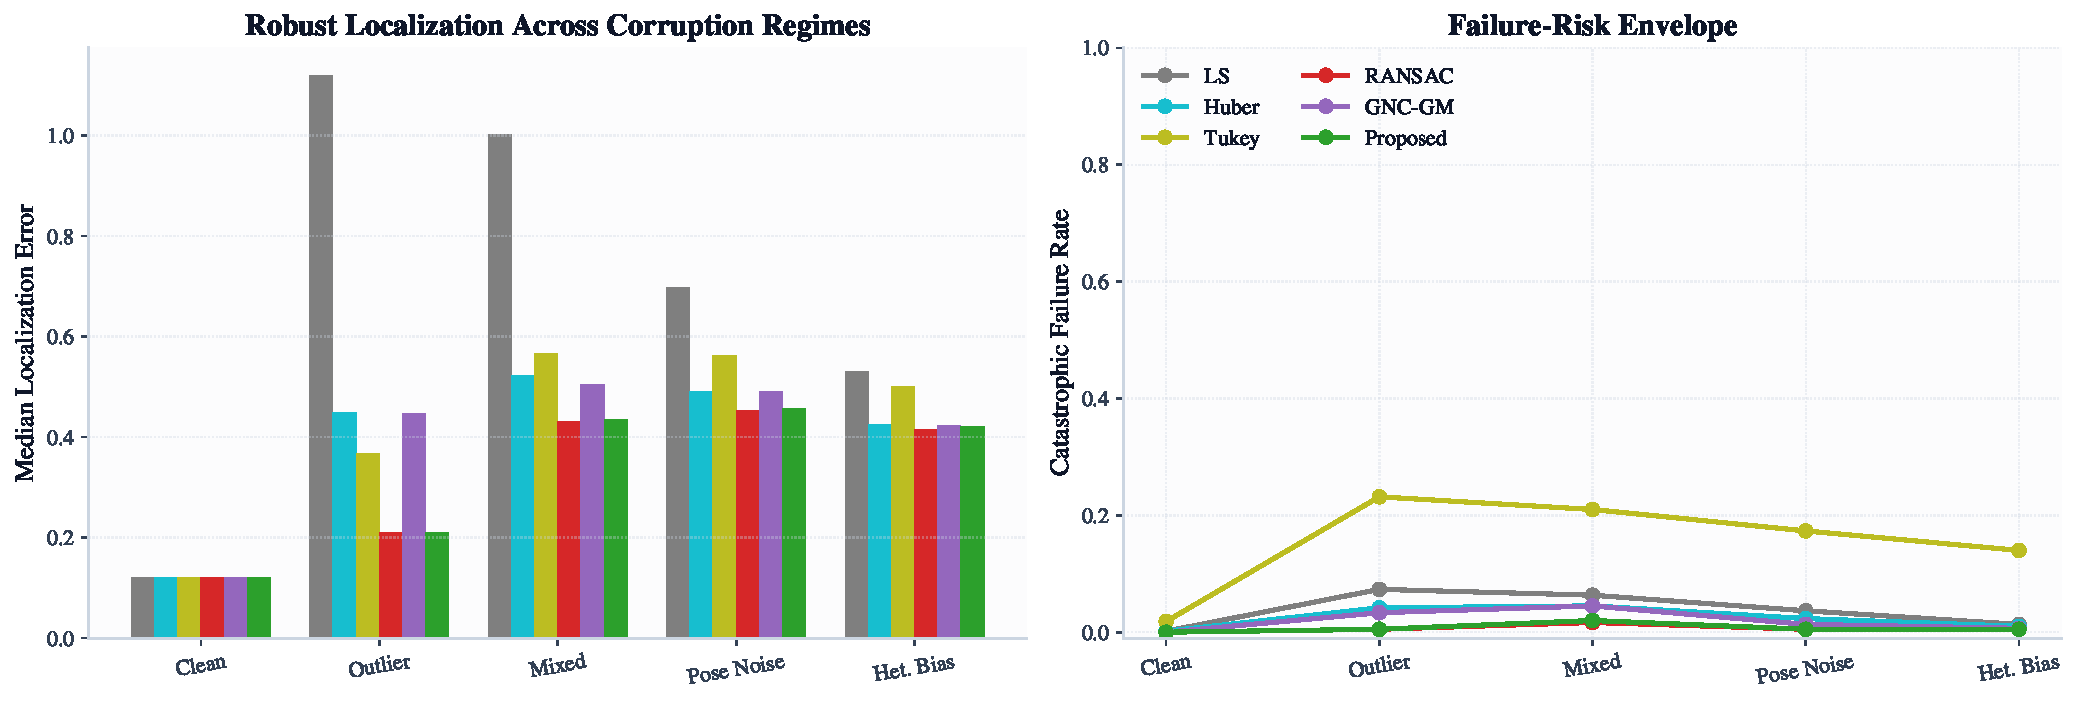
\includegraphics[width=0.98\linewidth]{../figures/figure_story_regimes}
\caption{Main corrupted-measurement benchmark. Left: median localization error across the five regimes. Right: catastrophic-failure rate. The proposed estimator is designed to suppress failure risk under corrupted bearing sets rather than to claim universal dominance in every possible regime.}
\label{fig:storyregimes}
\end{figure}

Figure~\ref{fig:storycdf} adds a distribution-level view for the two regimes in which the front-end story matters most. In the outlier-rich regime, the proposed estimator shifts the full error distribution leftward relative to least squares and GNC-GM, nearly overlapping RANSAC over most of the range. The 90th-percentile error drops from 2.5034 for least squares to 0.6697 for the proposed method, and the success rate at $0.1R$ increases from 0.4875 to 0.9400. In the mixed-corruption regime, the same pattern persists: the 90th percentile drops from 2.7369 to 1.0979 and the success rate increases from 0.5625 to 0.8925. This confirms that the gain is not restricted to a few easy trials or a few catastrophic outliers. The full empirical distribution is compressed, which is exactly what a robust front end should achieve before a downstream tracker or planner is invoked.

\begin{figure}[!htbp]
\centering
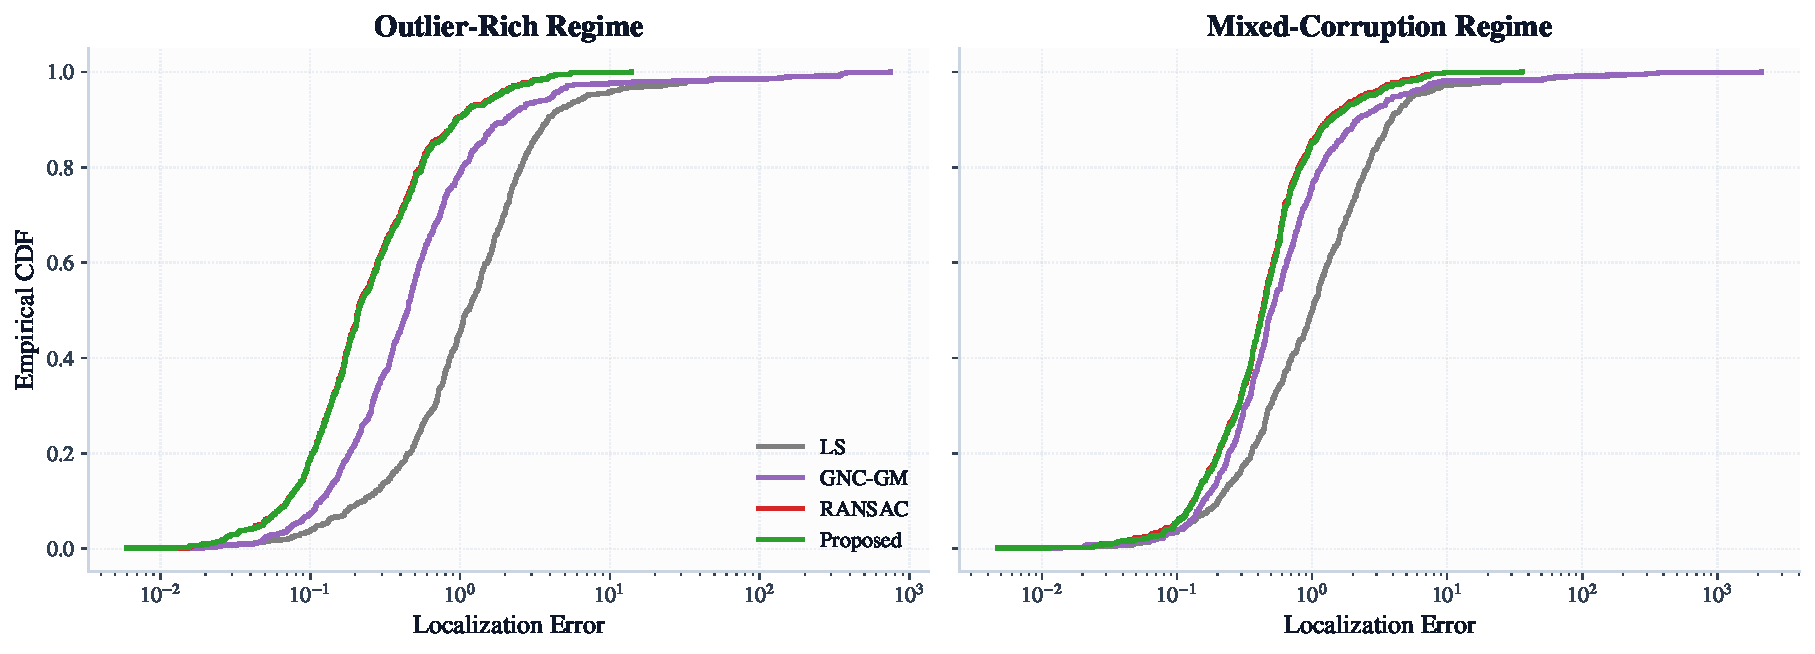
\includegraphics[width=0.98\linewidth]{../figures/figure_story_cdf}
\caption{Empirical CDFs in the outlier-rich and mixed-corruption regimes. The proposed estimator closely tracks the strongest robust baseline while shifting the overall error distribution left of least squares and GNC-GM, especially in the upper tail.}
\label{fig:storycdf}
\end{figure}

Figure~\ref{fig:thresholdsweep} and Table~\ref{tab:tailrisk} make the same point under stricter failure thresholds and paired tests. When the catastrophic threshold is tightened from $0.5R$ to $0.2R$, the outlier-regime failure rate drops from 0.1725 for least squares to 0.0375 for the proposed estimator, and the mixed-regime failure rate drops from 0.2000 to 0.0625. The paired Wilcoxon tests show stable gains over least squares and PSO in both hard regimes. The comparison against RANSAC is intentionally narrower: RANSAC is already strong in gross-outlier conditions, so the main gain of the proposed front-end is not to replace it everywhere, but to preserve the same robust-fusion pipeline when bias, missing data, and pose uncertainty appear together.

\begin{figure}[!htbp]
\centering
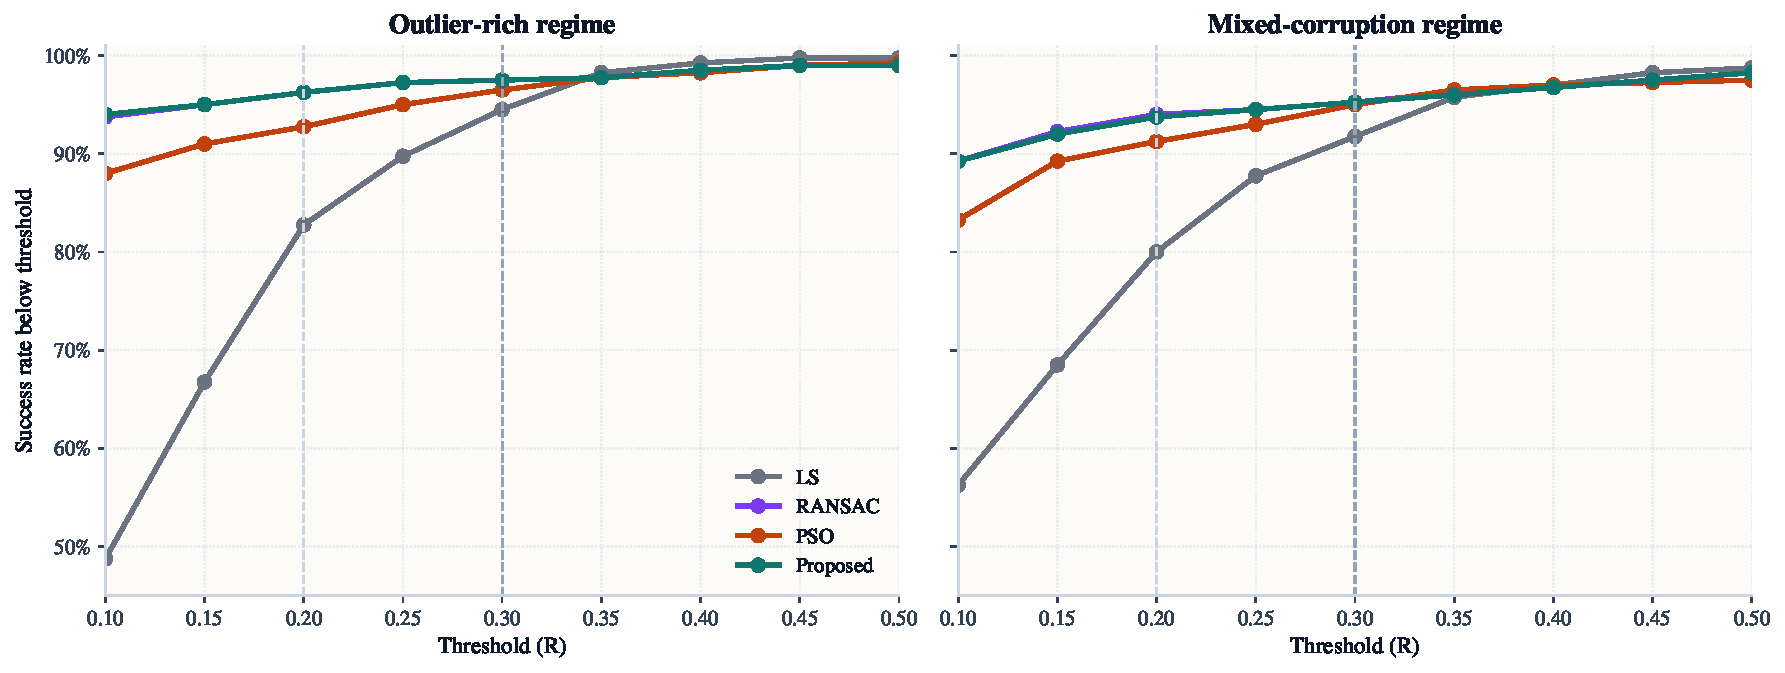
\includegraphics[width=0.98\linewidth]{../figures/figure_threshold_sweep}
\caption{Success-rate sweep under increasingly strict error thresholds. The proposed front end preserves a large margin over least squares as the acceptable cue radius contracts from $0.5R$ to $0.1R$.}
\label{fig:thresholdsweep}
\end{figure}

\begin{table}[!htbp]
\centering
\caption{Paired tail-risk and significance summary in the two most demanding synthetic regimes. Positive $\Delta$ indicates lower error for the proposed front-end.}
\label{tab:tailrisk}
\small
\resizebox{\linewidth}{!}{%
\begin{tabular}{llrrrrr}
\toprule
Regime & Comparison & Wins--Losses--Ties & Wilcoxon $p$ & Median $\Delta$ & P95 Baseline / Proposed & P99 Baseline / Proposed \\
\midrule
Outlier & Proposed vs LS     & 521--70--9   & $2.35\times 10^{-77}$ & 0.7637 & 6.9637 / 1.7526 & 159.7861 / 3.8781 \\
Outlier & Proposed vs RANSAC & 93--86--421  & 0.0357                & 0.0000 & 1.7049 / 1.7526 & 3.8781 / 3.8781 \\
Outlier & Proposed vs PSO    & 345--255--0  & $4.70\times 10^{-4}$  & 0.0248 & 3.6427 / 1.7526 & 663.2234 / 3.8781 \\
\midrule
Mixed   & Proposed vs LS     & 411--169--20 & $2.39\times 10^{-42}$ & 0.3258 & 5.5785 / 2.5071 & 76.1232 / 6.7965 \\
Mixed   & Proposed vs RANSAC & 78--107--415 & 0.9992                & 0.0000 & 2.3245 / 2.5071 & 6.4788 / 6.7965 \\
Mixed   & Proposed vs PSO    & 410--190--0  & $5.11\times 10^{-23}$ & 0.1058 & 4.1567 / 2.5071 & 1334.8015 / 6.7965 \\
\bottomrule
\end{tabular}}
\end{table}


\subsection{Why Not Just RANSAC?}

RANSAC is the right baseline to confront directly because it is already very effective in pure gross-outlier regimes. The results above show that the proposed estimator does not materially outperform RANSAC in the outlier benchmark, and that is an important boundary condition for the paper. The motivation for keeping the proposed front-end is different: the same pipeline must also remain stable when heterogeneous bias, pose uncertainty, and partial trimming interact with gross corruption. In those regimes, the proposed estimator maintains slightly lower medians than RANSAC and uses the same downstream robust-refinement stack as the rest of the manuscript.

Figure~\ref{fig:ransaccase} illustrates one representative heterogeneous-bias case from the benchmark. Several bearings are individually plausible, but one strongly biased ray pulls the consensus solution away from the target. RANSAC keeps a front-end cue with 1.0768 error, while the proposed estimator trims the most inconsistent bearing and reduces the error to 0.5100. The point is specific but useful for multi-error sensing: once bias and measurement inconsistency coexist, a consensus-only front end can still benefit from trimmed reweighting and selective suppression of the most harmful bearings.

\begin{figure}[!htbp]
\centering
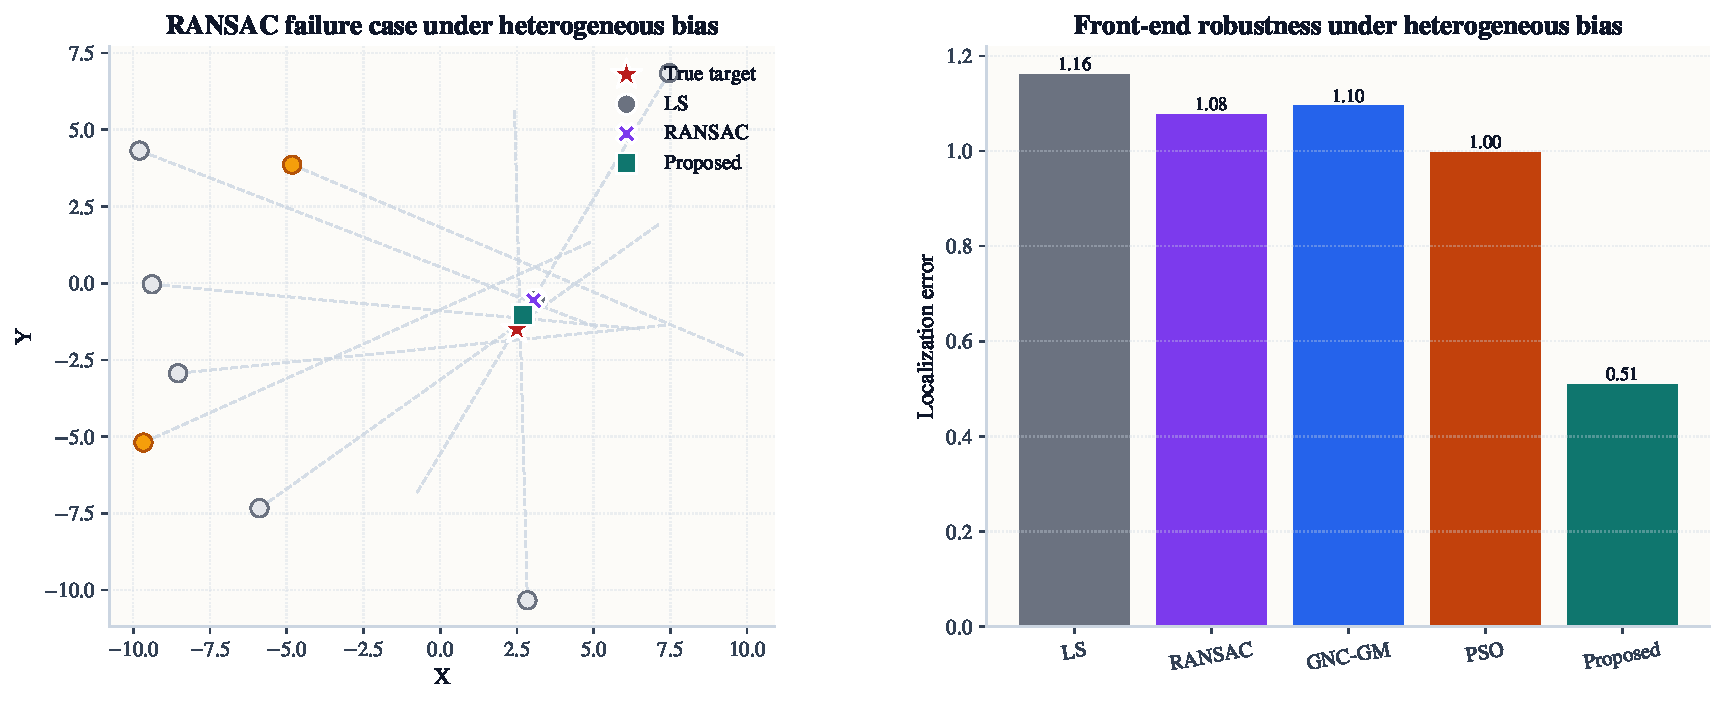
\includegraphics[width=0.98\linewidth]{../figures/figure_ransac_failure_case}
\caption{Representative heterogeneous-bias case in which consensus alone is insufficient. The proposed front end retains the same robust-estimation stack used in the main benchmark and suppresses a strongly biased bearing that pulls the RANSAC cue away from the target.}
\label{fig:ransaccase}
\end{figure}

\subsection{Fixed-Budget Screening Is Conditional, Not Universal}

The screening benchmark confirms a conditional story. All-sensor robust fusion remains the unconstrained upper bound, with overall median error 0.4003. Under fixed subset budgets, however, screening is still useful. The proposed geometry--reliability policy improves the overall median error from 0.5572 for residual-only screening and 0.6294 for reliability-only screening to 0.5015. The adaptive variant reduces the overall median further to 0.4723 and improves the severe-regime median from 0.7491 to 0.7291 (Table~\ref{tab:screening}).

\begin{table}[!htbp]
\centering
\caption{Fixed-budget screening benchmark. The all-sensor robust estimator remains the unconstrained upper bound, whereas adaptive and geometry--reliability screening improve over residual-only and reliability-only screening under fixed subset budgets.}
\label{tab:screening}
\small
\resizebox{\linewidth}{!}{%
\begin{tabular}{lrrrrrr}
\toprule
Policy & Overall Median & Mixed Median & Severe Median & Success@1.0 & Cat.@5.0 & Wins--Losses \\
\midrule
All-Sensor Robust & 0.4003 & 0.2759 & 0.6451 & 0.8444 & 0.0297 & -- \\
Residual-Only     & 0.5572 & 0.4204 & 0.7873 & 0.8258 & 0.0303 & 396--670 \\
Reliability-Only  & 0.6294 & 0.5077 & 0.8236 & 0.8124 & 0.0297 & 366--777 \\
Geom+Reliability  & 0.5015 & 0.3335 & 0.7491 & 0.8211 & 0.0286 & 454--739 \\
Adaptive          & 0.4723 & 0.2994 & 0.7291 & 0.8275 & 0.0286 & 97--247$^{a}$ \\
\bottomrule
\end{tabular}}

\vspace{0.4em}
\noindent\footnotesize{$^{a}$ Wins--losses for Adaptive report the paired comparison against the proposed always-on screening policy; adaptive screening ties in 1372 of 1716 fixed-budget cases and therefore acts mainly as a conservative gate rather than as a universal replacement for all-sensor fusion.}
\end{table}


The paired counts clarify the same point. The proposed always-on screening policy beats the residual-only baseline in 670 cases and loses in 396, with 650 ties. Against the all-sensor robust estimator, however, the same policy loses in 882 cases. Adaptive screening behaves more conservatively: it ties the always-on screening policy in 1372 of 1716 cases and improves the median error slightly by refusing to screen when the current bearing set does not appear heterogeneous enough. The benefit map in Figure~\ref{fig:benefitmap} shows the same behavior over the outlier-rate/budget plane: screening helps most when the budget is tight and measurement credibility is uneven.

\begin{figure}[!htbp]
\centering
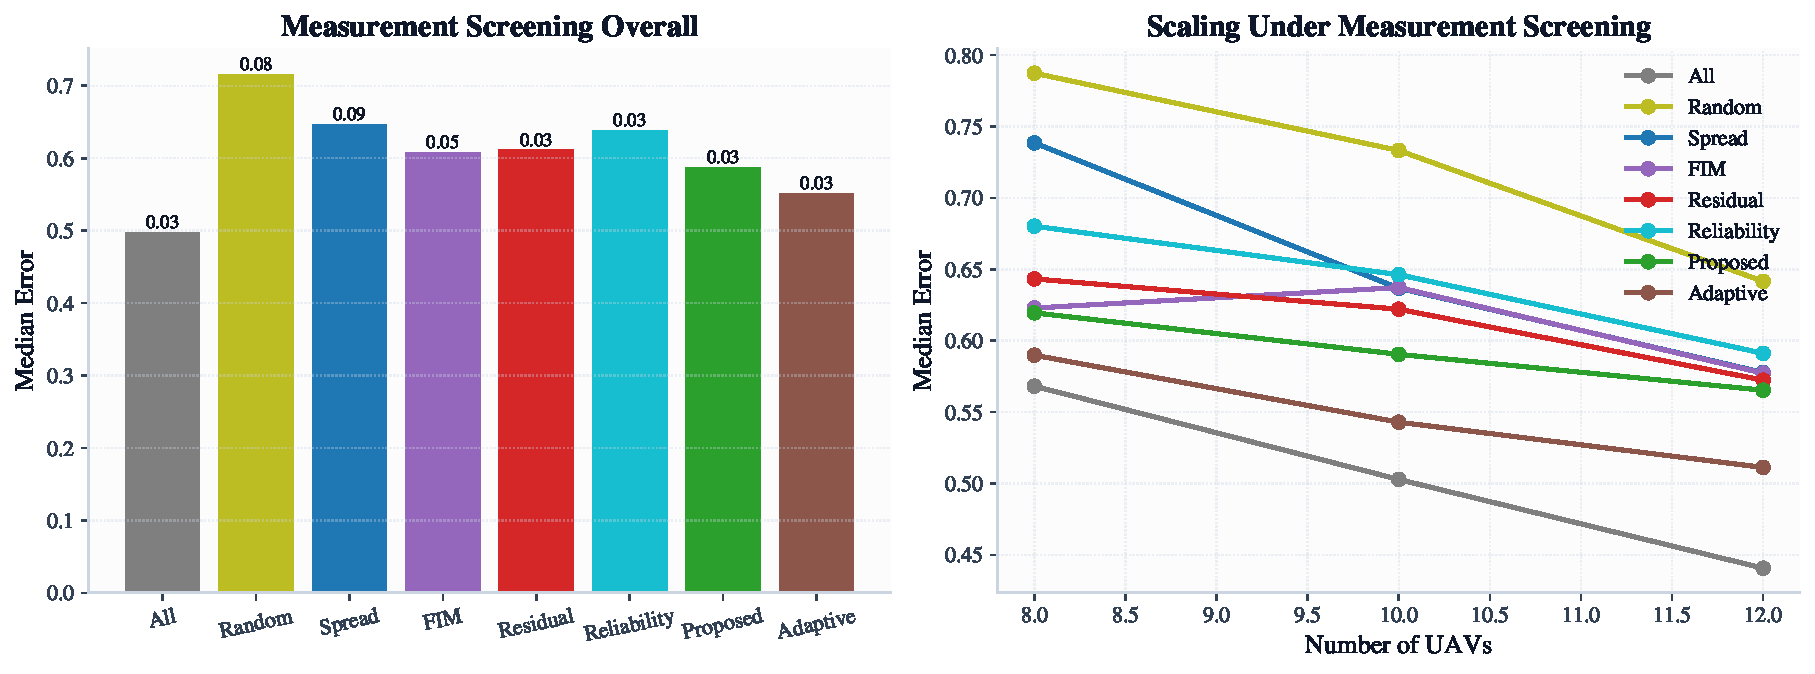
\includegraphics[width=0.98\linewidth]{../figures/figure_active_selection}
\caption{Fixed-budget screening benchmark over mixed and severe regimes. The all-sensor robust estimator remains the upper bound without budget constraints, while adaptive and geometry--reliability screening improve over simpler subset policies.}
\label{fig:screening}
\end{figure}

\begin{figure}[!htbp]
\centering
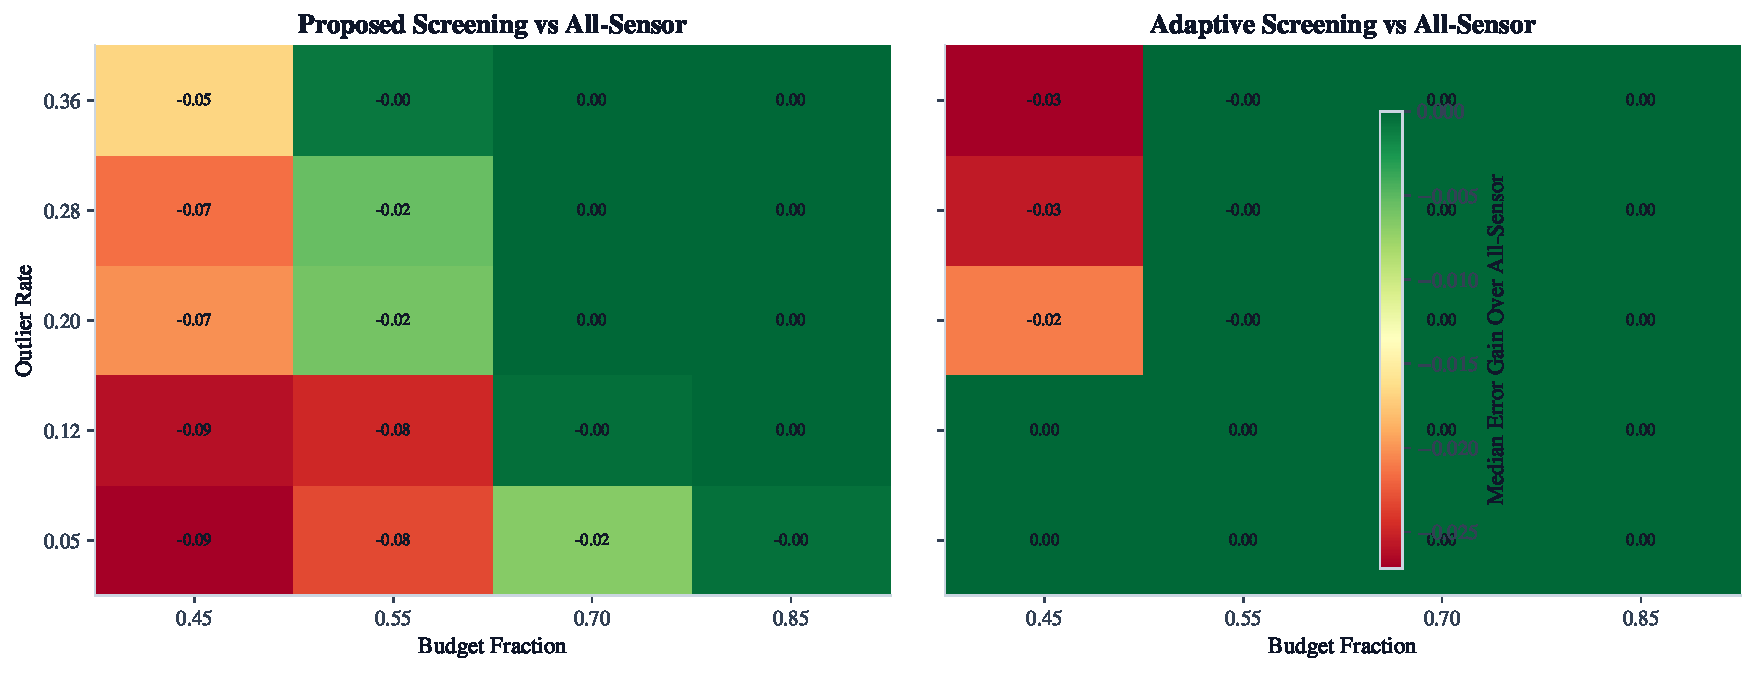
\includegraphics[width=0.86\linewidth]{../figures/figure_selection_benefit_map}
\caption{Selection benefit map under varying outlier rate and subset budget. The heat map shows the median error gain relative to all-sensor robust fusion, making clear that screening should be activated selectively rather than treated as a universal improvement.}
\label{fig:benefitmap}
\end{figure}

Figure~\ref{fig:screeningcases} turns the conditional interpretation into two concrete case studies. In the first case, a severe perturbed 10-observer window with budget $k=5$, the proposed subset policy attains error 0.4987, while residual-only and reliability-only selection both remain at 1.1800 and spread-only and CRLB-only heuristics remain at 1.9091. The all-sensor robust estimator is still slightly better at 0.4319, which is why the screening module is framed as a fixed-budget tool rather than as a replacement for full-set fusion. In the second case, a severe random 10-observer window with budget $k=4$, always-on screening would be the wrong decision: all-sensor robust fusion already achieves error 0.2750, while the always-on geometry--reliability policy degrades to 1.4929. The adaptive gate keeps the full set in that second case and therefore preserves the 0.2750 error. Together, these examples show why the adaptive gate is needed when the full set is already reliable.

\begin{figure}[!htbp]
\centering
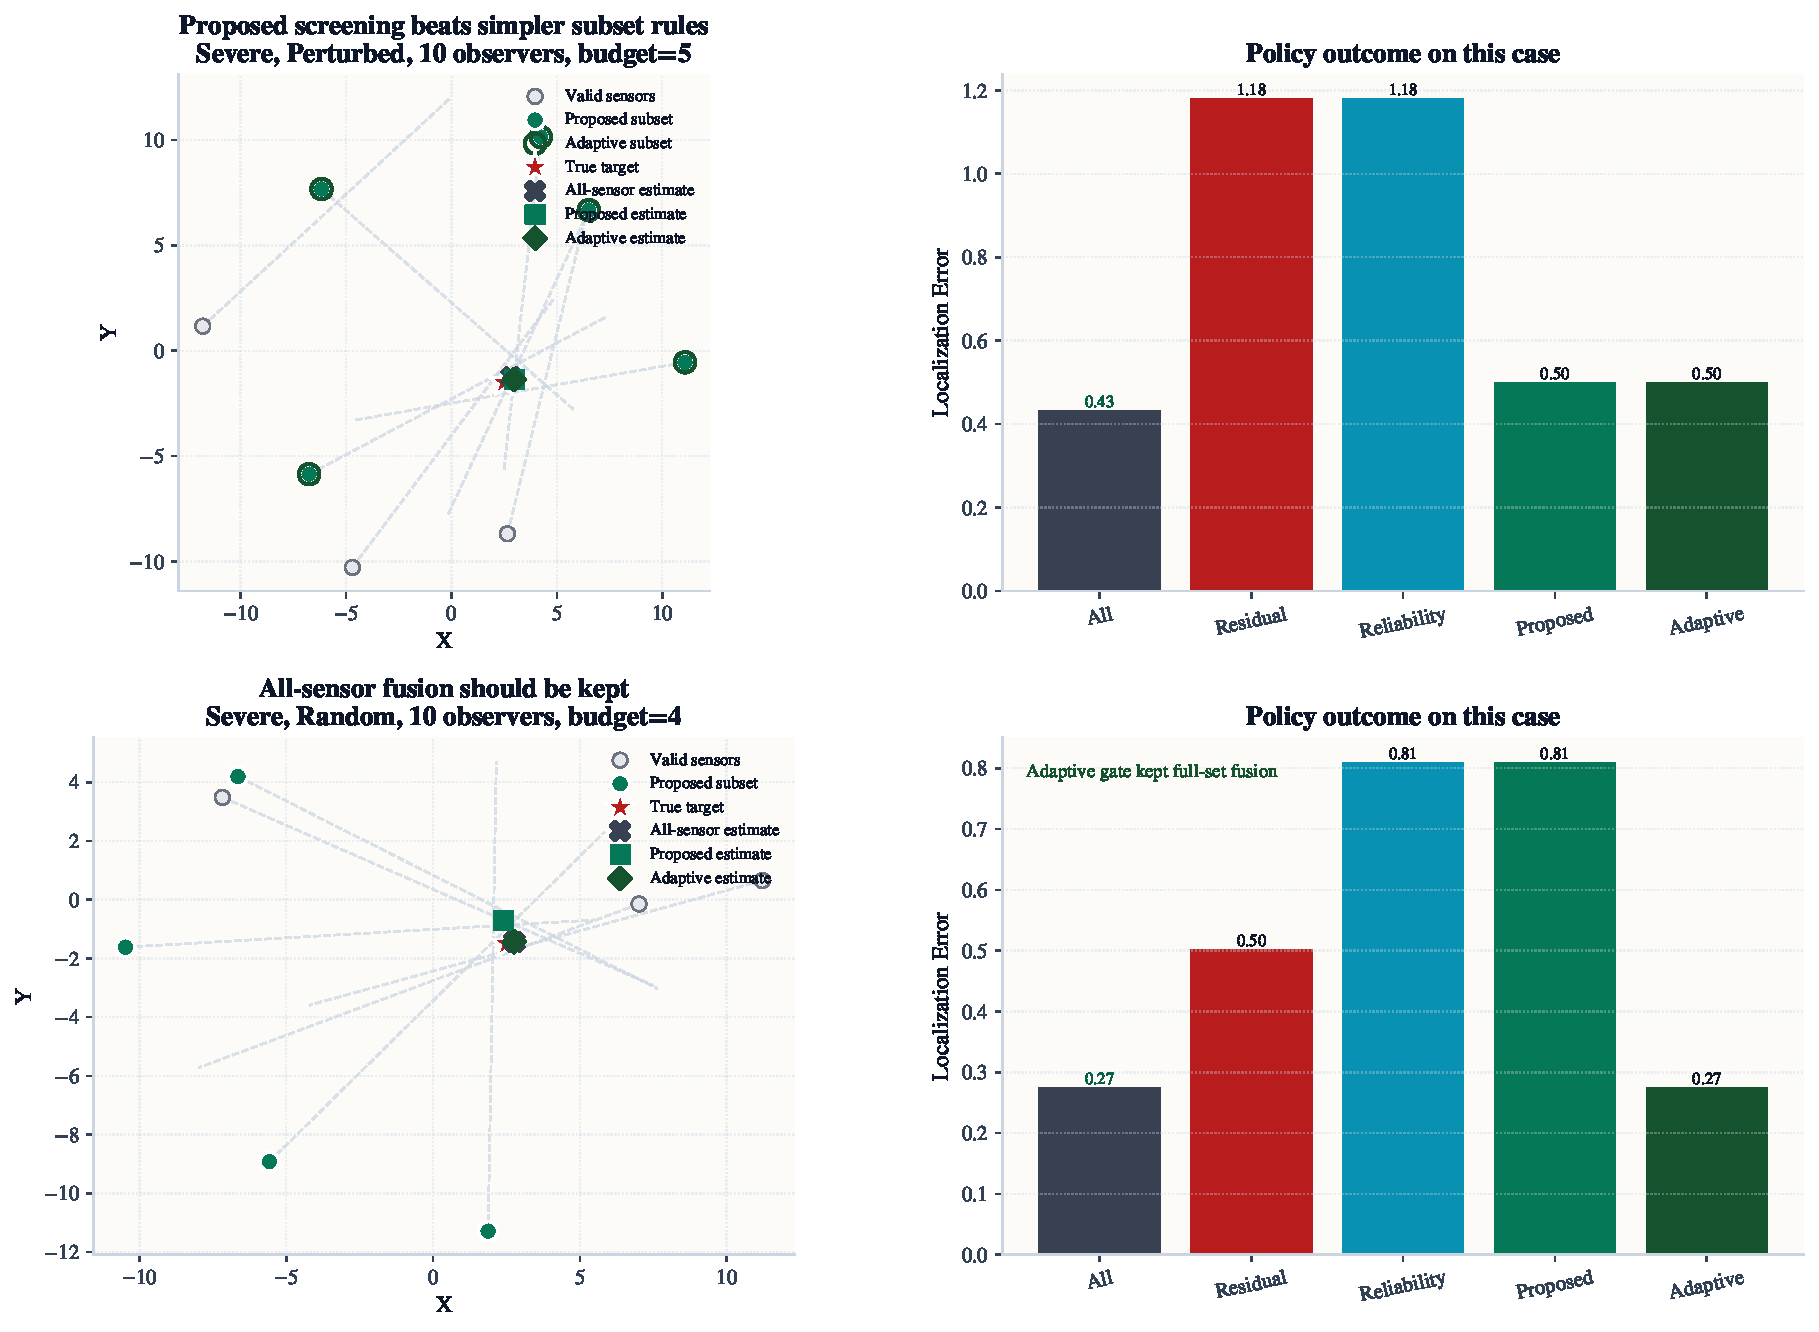
\includegraphics[width=0.98\linewidth]{../figures/figure_screening_cases}
\caption{Case studies for fixed-budget screening. Top: a severe window in which the proposed geometry--reliability subset clearly outperforms simpler fixed-budget heuristics, although the unconstrained all-sensor solution remains slightly better. Bottom: a severe window in which all-sensor fusion should be retained, and the adaptive gate correctly avoids unnecessary pruning.}
\label{fig:screeningcases}
\end{figure}

Figure~\ref{fig:screeningweights} addresses the most obvious methodological concern about the screening score: whether a nearby coefficient vector would change the conclusion completely. On the exact $0.8\times/1.0\times/1.2\times$ perturbation grid for the four normalized coefficients, the median error across the 81 combinations is 0.5278, compared with 0.5269 for the default setting. The 5th--95th percentile interval spans only 0.5253--0.5412, and the median Jaccard overlap with the default selected subset remains 0.9840. These results do not make the score optimal, but they do show that the reported behavior is not a brittle artifact of one manually tuned coefficient vector.

\begin{figure}[!htbp]
\centering
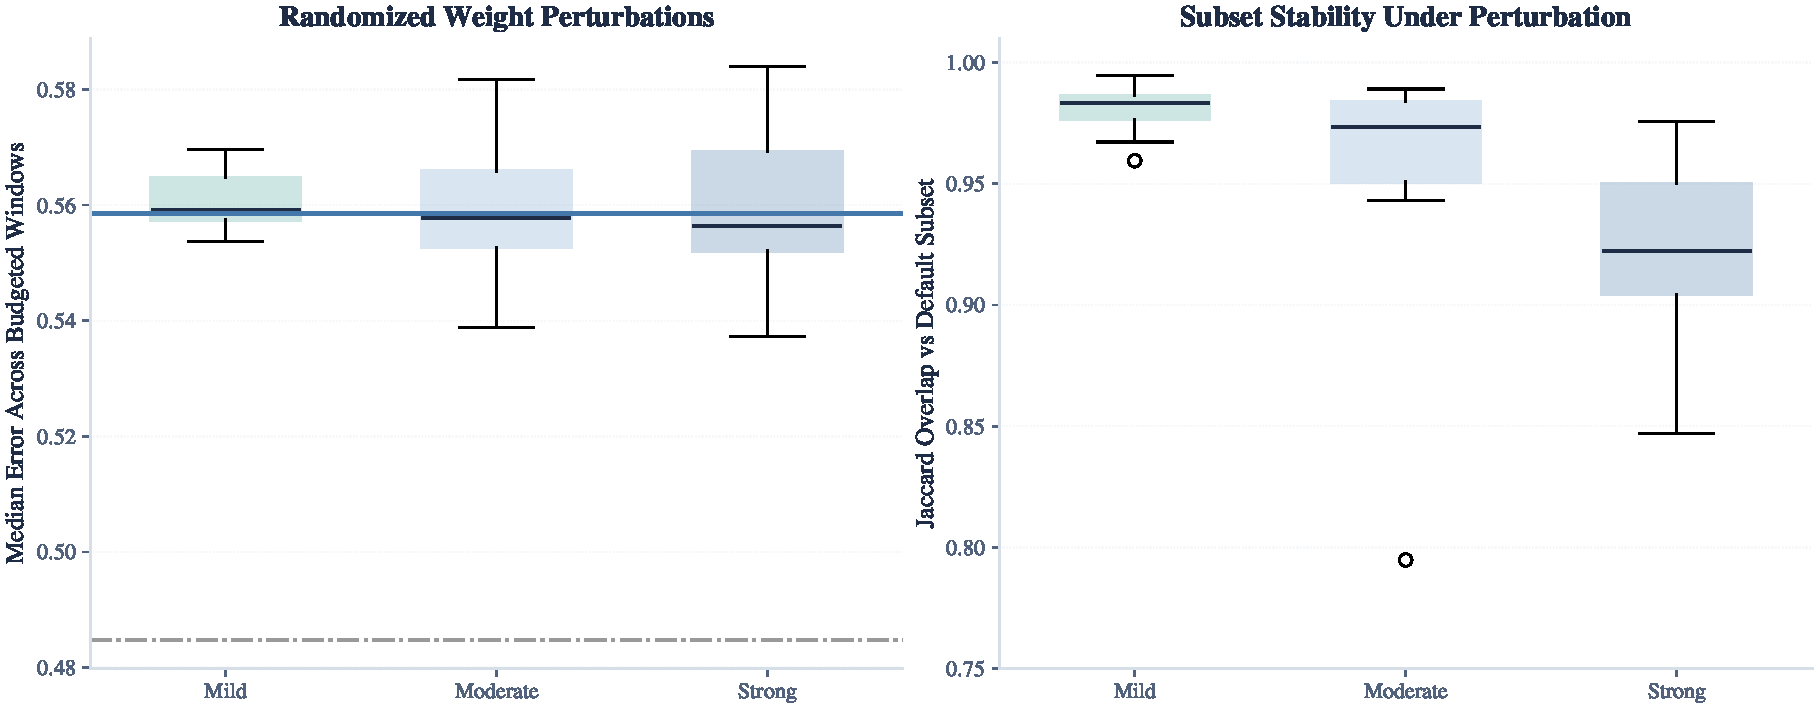
\includegraphics[width=0.98\linewidth]{../figures/figure_screening_weight_sensitivity}
\caption{Sensitivity of the screening module under the exact $\pm20\%$ coefficient grid. The budgeted median error remains close to the default setting, and the selected subsets stay strongly aligned with the default policy.}
\label{fig:screeningweights}
\end{figure}

\subsection{Pseudo-Physical Dynamic Replay}

The pseudo-physical replay results show that the revised estimator is not only a static synthetic benchmark result. In the mild dynamic setting, the median error decreases from 0.1603 for least squares to 0.1373 for the proposed method, and the success rate at the 1.0 threshold reaches 1.0. In the harsh dynamic setting, the median error decreases from 0.4979 to 0.3498, while the 90th-percentile error drops from 1.5877 to 0.6505 (Table~\ref{tab:pseudophysical}). The proposed method remains close to RANSAC in the mild setting and slightly better in the harsh setting, which is consistent with the main Monte Carlo story: consensus is important, but the additional trimmed refinement becomes more valuable when corruption sources combine.

\begin{table}[!htbp]
\centering
\caption{Pseudo-physical dynamic replay validation with delay, attitude jitter, and per-sensor bias. The proposed method is competitive with RANSAC in the mild setting and slightly better in the harsh setting while remaining clearly stronger than least squares and GNC-GM.}
\label{tab:pseudophysical}
\begin{tabular}{llrrrr}
\toprule
Regime & Method & Median & P90 & Success@1.0 & Cat.@5.0 \\
\midrule
Mild Dynamic  & Least Squares & 0.1603 & 0.6367 & 0.9722 & 0.0000 \\
Mild Dynamic  & GNC-GM        & 0.1496 & 0.3004 & 1.0000 & 0.0000 \\
Mild Dynamic  & RANSAC        & 0.1334 & 0.2635 & 1.0000 & 0.0000 \\
Mild Dynamic  & Proposed      & 0.1373 & 0.2659 & 1.0000 & 0.0000 \\
\midrule
Harsh Dynamic & Least Squares & 0.4979 & 1.5877 & 0.7528 & 0.0028 \\
Harsh Dynamic & GNC-GM        & 0.3647 & 0.7505 & 0.9694 & 0.0028 \\
Harsh Dynamic & RANSAC        & 0.3559 & 0.6505 & 0.9778 & 0.0056 \\
Harsh Dynamic & Proposed      & 0.3498 & 0.6505 & 0.9750 & 0.0056 \\
\bottomrule
\end{tabular}
\end{table}


\subsection{Ablation and Sensitivity Trends}

The ablation study helps explain why the method behaves like a front-end stack rather than like a single robustifier. In the mixed regime, removing trimming degrades the median error from 0.6779 to 0.7350 and inflates the 90th percentile from 1.5705 to 3.1809, showing that trimming is important mainly for suppressing the tail rather than for changing the average case. By contrast, removing common-bias estimation only changes the median slightly in that regime, which is consistent with the main story: the dominant gain comes from rejecting badly corrupted bearings, while bias correction becomes more helpful in structured bias regimes. Figure~\ref{fig:ablation} visualizes the same trend and supports a narrower interpretation of the module contributions.

The sensitivity sweeps tell a similarly nuanced story. As the outlier rate increases from 0.0 to 0.4, the proposed estimator stays below least squares throughout and remains below PSO at the hardest outlier settings. Under increasing common bias, however, the gap narrows and PSO becomes competitive at the largest tested bias values. Under nominal-noise increase, the proposed estimator again remains clearly below least squares and is comparable to or slightly better than PSO at higher noise levels. The front-end is therefore strongest in outlier-rich and mixed-corruption settings rather than under every possible disturbance model.

\begin{figure}[!htbp]
\centering
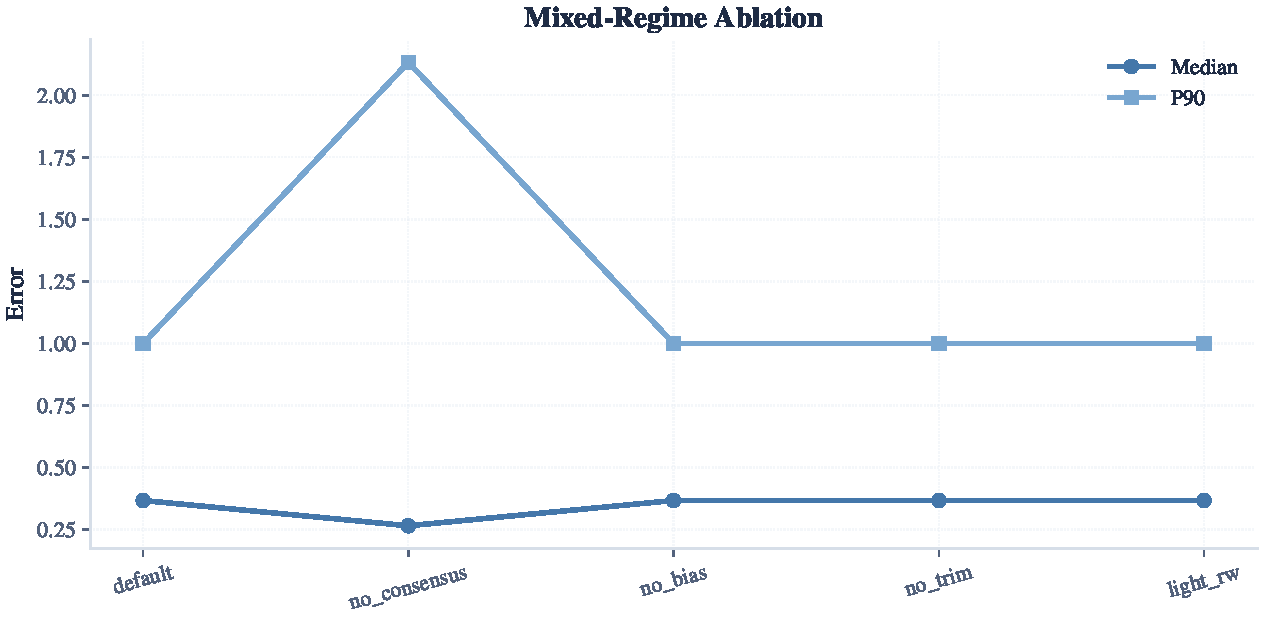
\includegraphics[width=0.82\linewidth]{../figures/figure_ablation_mixed}
\caption{Mixed-regime ablation. The main effect of trimming and iterative reweighting is a reduction in tail risk rather than a dramatic change in easy cases.}
\label{fig:ablation}
\end{figure}

\begin{figure}[!htbp]
\centering
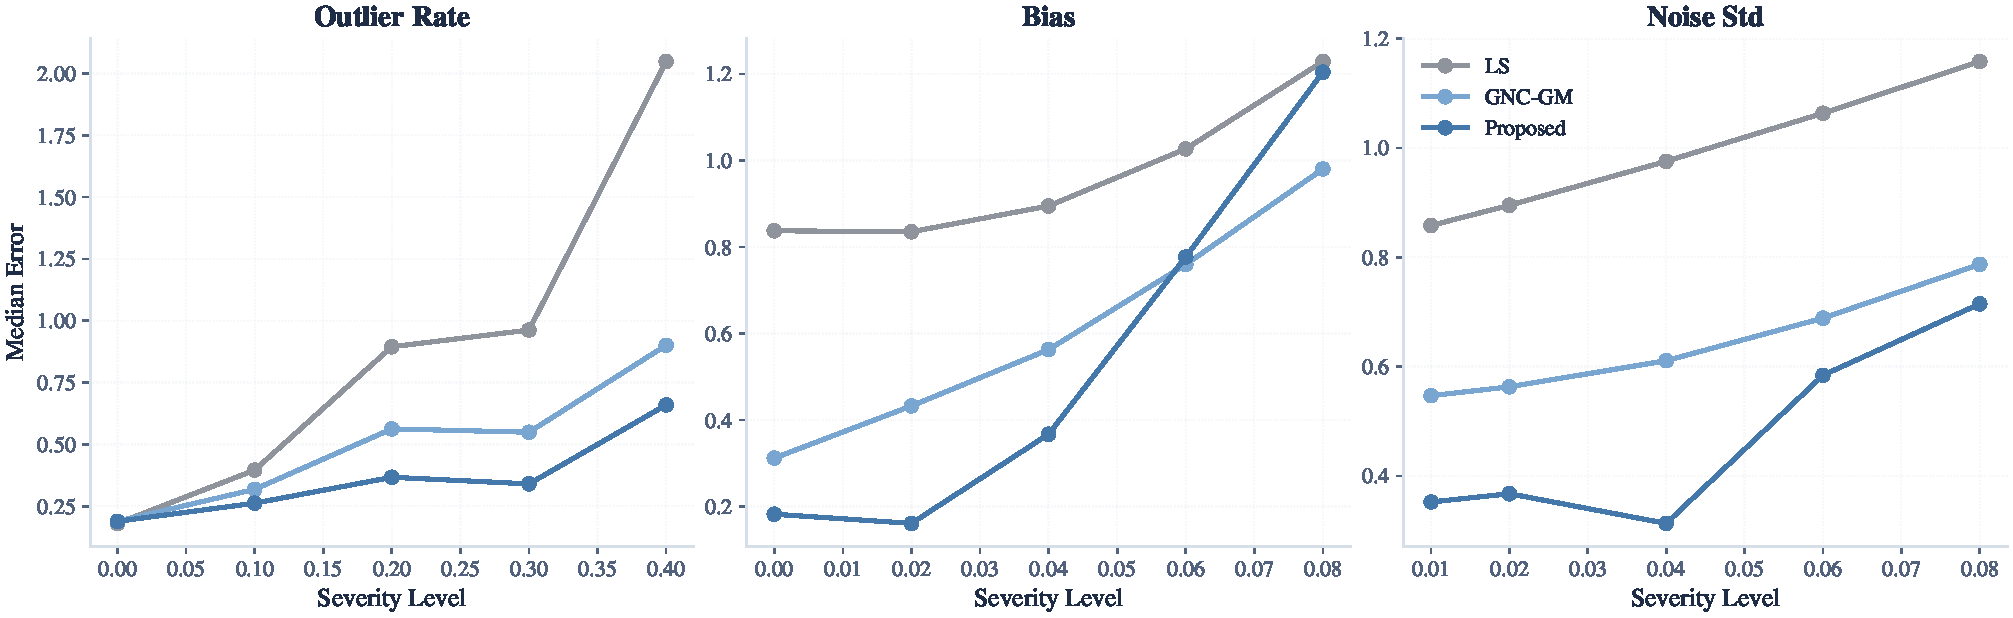
\includegraphics[width=0.98\linewidth]{../figures/figure_sensitivity_sweep}
\caption{Sensitivity sweeps over outlier rate, bias magnitude, and nominal noise. The proposed estimator remains clearly stronger than least squares, while its advantage over PSO depends on the corruption type.}
\label{fig:sensitivity}
\end{figure}

\subsection{Formation, Observability, and Sensor-Count Generalization}

The formation study confirms that the proposed front end is not tied to one nominal geometry. Across circle, ellipse, perturbed, and random formations, the proposed estimator reduces the median error relative to least squares in every tested case (Appendix~C, Table~\ref{tab:formationextra}). The largest gain appears in the random formation, where the median drops from 2.1047 to 0.5768. The method is not uniformly best against every stronger baseline: PSO remains competitive in some formation families, especially when the geometry is already favorable. The main advantage appears when corrupted bearings destabilize otherwise reasonable geometry.

Sensor-count scaling shows a similar pattern. The proposed estimator benefits substantially from moving from 4 to 8 or 10 observers, especially in random formations where the median decreases from 0.7221 at 4 observers to 0.4051 at 10 observers. The circle-formation scaling curve is also informative: the least-squares median is non-monotonic and can become worse at 12 observers under corruption, whereas the robust front end remains below 0.45 once eight or more observers are available. This suggests that additional corrupted measurements do not automatically help unless the fusion rule is robust.

The observability analysis adds an important nuance. Better isotropy still correlates with lower median error, but poor geometry alone does not explain the failures of least squares. Figure~\ref{fig:observability} shows that the proposed front end compresses the vertical spread of the error distribution over a wide isotropy range, meaning that it is addressing corrupted measurements rather than merely exploiting easy geometry.

\begin{figure}[!htbp]
\centering
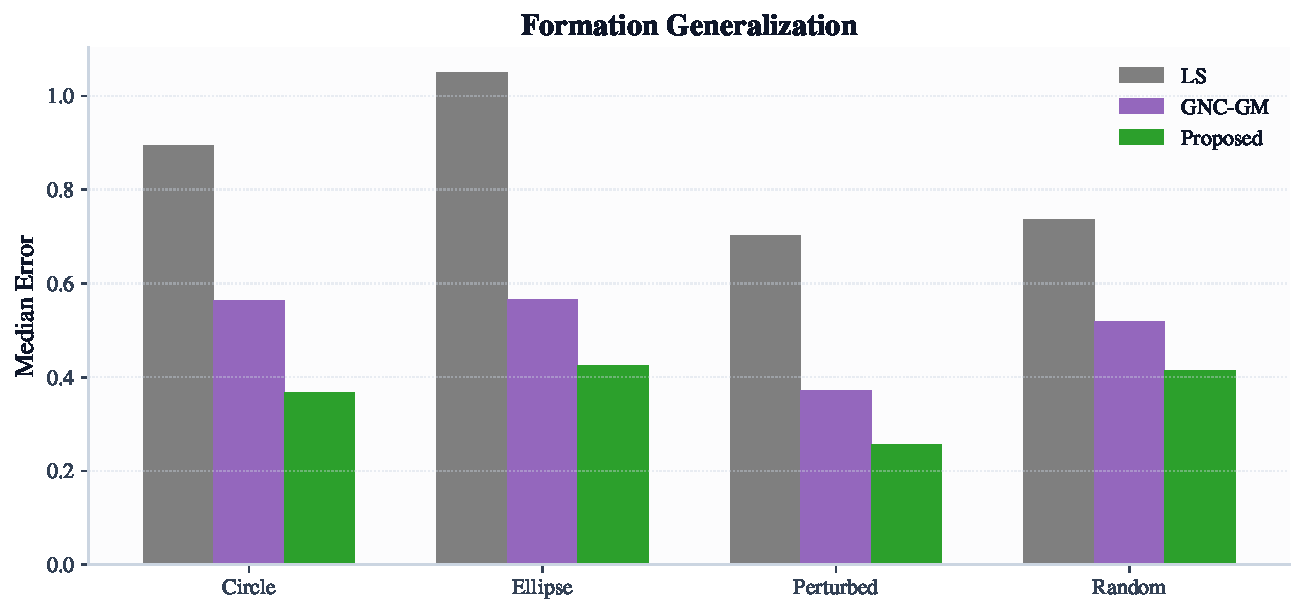
\includegraphics[width=0.82\linewidth]{../figures/figure_formation_generalization}
\caption{Formation generalization under mixed corruption. The proposed estimator is consistently below least squares across circle, ellipse, perturbed, and random formations.}
\label{fig:formation}
\end{figure}

\begin{figure}[!htbp]
\centering
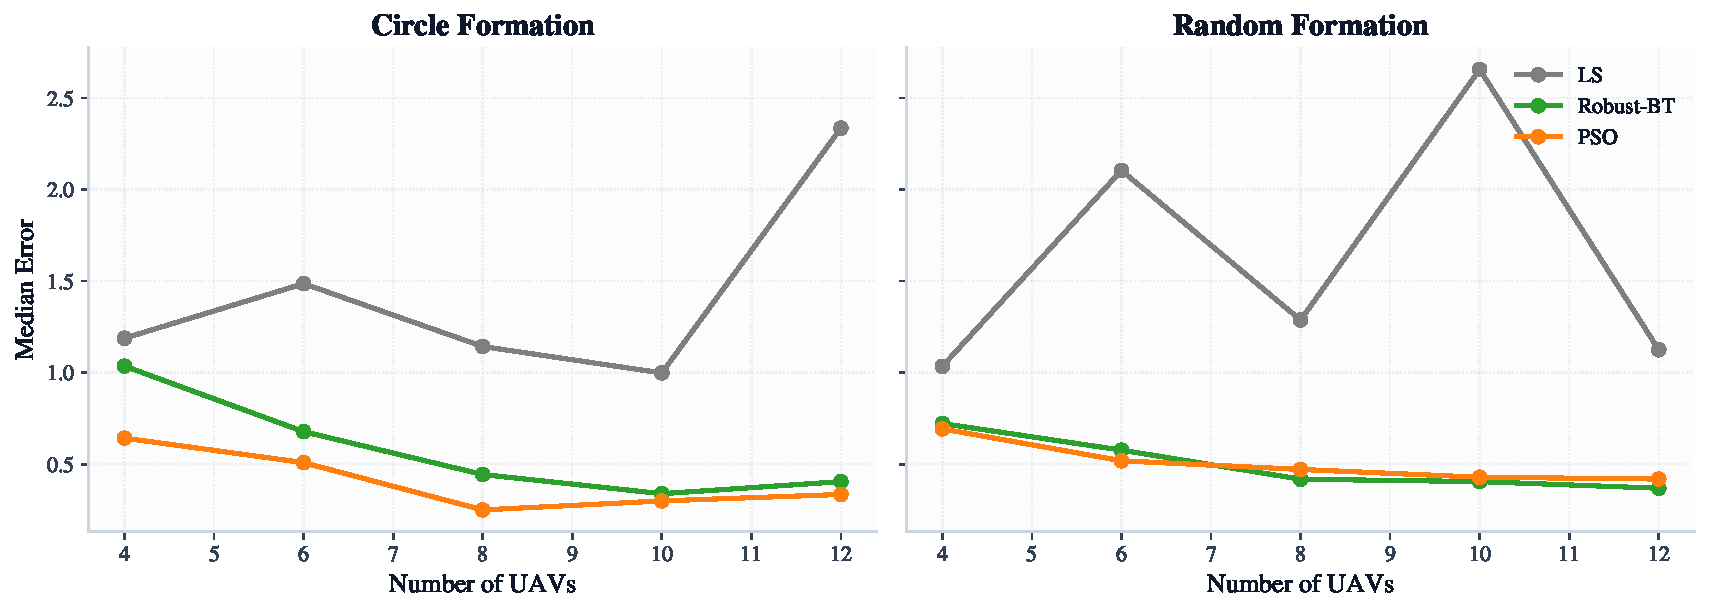
\includegraphics[width=0.98\linewidth]{../figures/figure_scaling}
\caption{Sensor-count scaling for circle and random formations. Robust fusion becomes substantially more stable once eight or more observers are available.}
\label{fig:scaling}
\end{figure}

\begin{figure}[!htbp]
\centering
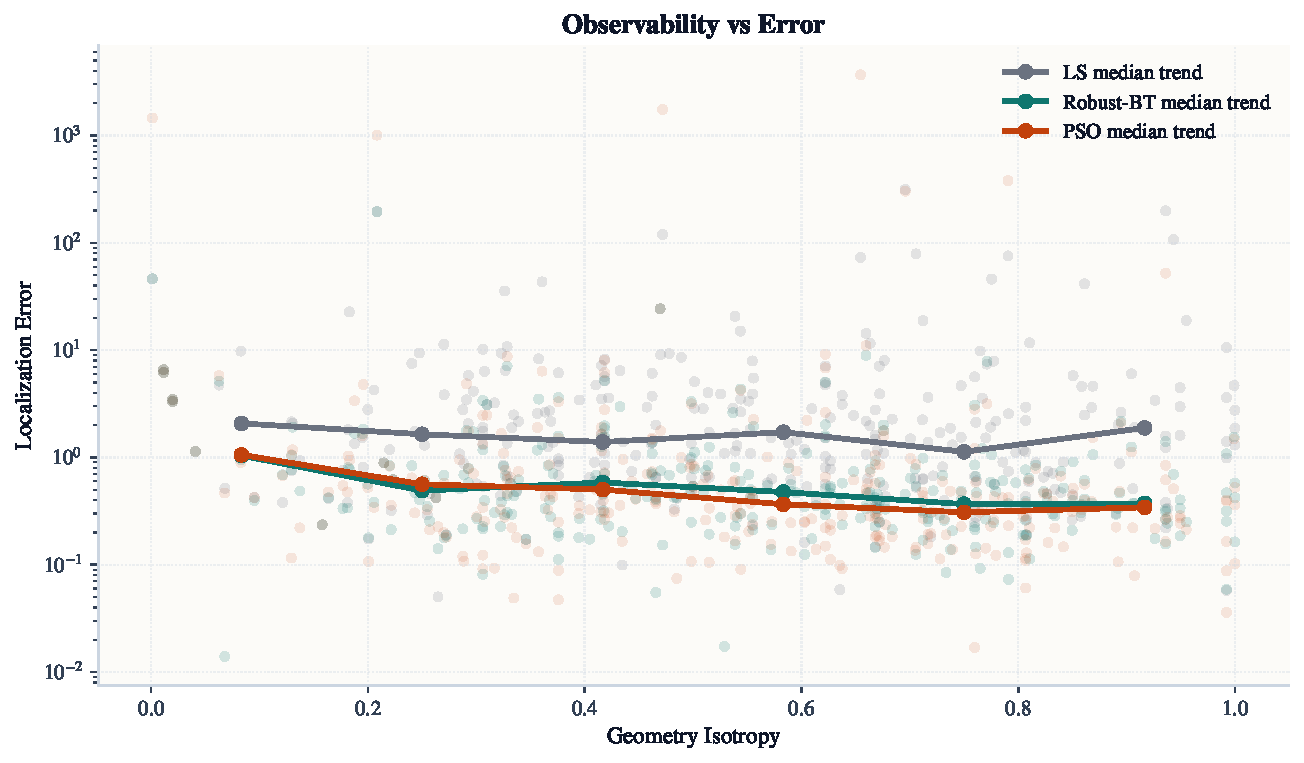
\includegraphics[width=0.90\linewidth]{../figures/figure_observability}
\caption{Error versus geometry isotropy. The proposed front end narrows the error spread even when the geometry is not especially favorable.}
\label{fig:observability}
\end{figure}

\subsection{PyBullet Multi-Vehicle Replay}

The PyBullet replay layer provides the strongest evidence in the current manuscript that the story is not limited to static point sets. Table~\ref{tab:pybulletparams} summarizes the replay configuration, including update rate, delay distribution, attitude-induced perturbation, and gust disturbance. Over 1844 replayed localization cycles, the overall median error decreases from 4.4387 for least squares to 1.1539 for the proposed estimator, while the catastrophic-failure rate drops from 0.4675 to 0.1605 (Appendix~C, Table~\ref{tab:pybullet}). In the nominal replay regime, the median decreases from 3.1608 to 0.8483; in the disturbed regime, it decreases from 5.4216 to 1.6113. The 90th percentile is reduced from 31.7371 to 7.8292 overall, which indicates that the gain is driven as much by tail suppression as by average-case improvement.

\begin{table}[!htbp]
\centering
\caption{PyBullet replay configuration used for the semi-physical multi-UAV validation layer. Localization windows are sampled every three control steps, corresponding to a 16~Hz cue-update rate.}
\label{tab:pybulletparams}
\small
\begin{tabularx}{\linewidth}{>{\RaggedRight\arraybackslash}p{0.28\linewidth} >{\RaggedRight\arraybackslash}p{0.18\linewidth} X}
\toprule
Parameter group & Setting & Value used in replay \\
\midrule
Vehicle simulator & Physics engine & \texttt{gym-pybullet-drones} with \texttt{PYB\_GND\_DRAG\_DW} physics \\
Timing & Simulation / control / localization rates & 240~Hz simulation, 48~Hz control, 16~Hz localization window update \\
Formation replay & Swarm layouts and counts & Circle and ellipse formations with 8 or 10 vehicles \\
Motion envelope & Orbit and altitude & 7.0--7.5~s replay horizon, 6.0~s orbit period, 0.95~m base altitude with 0.04~m stagger \\
Delay perturbation & Delay-step distribution & Mean 0.25 / 0.30 control steps, standard deviation 0.15 / 0.20 in nominal / disturbed replay \\
Attitude-induced corruption & Attitude and yaw-rate gains & 0.014 / 0.016 attitude gain and 0.0012 / 0.0015 yaw-rate gain in nominal / disturbed replay \\
Bias process & Common bias and drift & 0.004 / 0.005 shared bias with 0.0015 / 0.002 sinusoidal drift \\
Random corruption & Missing rate and outlier rate & 0.004 / 0.005 missing rate and 0.004 / 0.005 outlier rate in nominal / disturbed replay \\
Outlier magnitude & Outlier scale & 0.04 / 0.05 radians in nominal / disturbed replay \\
Gust disturbance & Gust force standard deviation & 0.11 / 0.12 with 0.20 / 0.22 trigger probability in nominal / disturbed replay \\
\bottomrule
\end{tabularx}
\end{table}


These results do not make the manuscript a field-validation paper, but they do move it beyond a purely static algorithm study. The replay benchmark incorporates multi-vehicle trajectories, timing variation, gust-like perturbation, and bias drift, and therefore provides a stronger link between synthetic geometry and UAV-like dynamics.

\begin{figure}[!htbp]
\centering
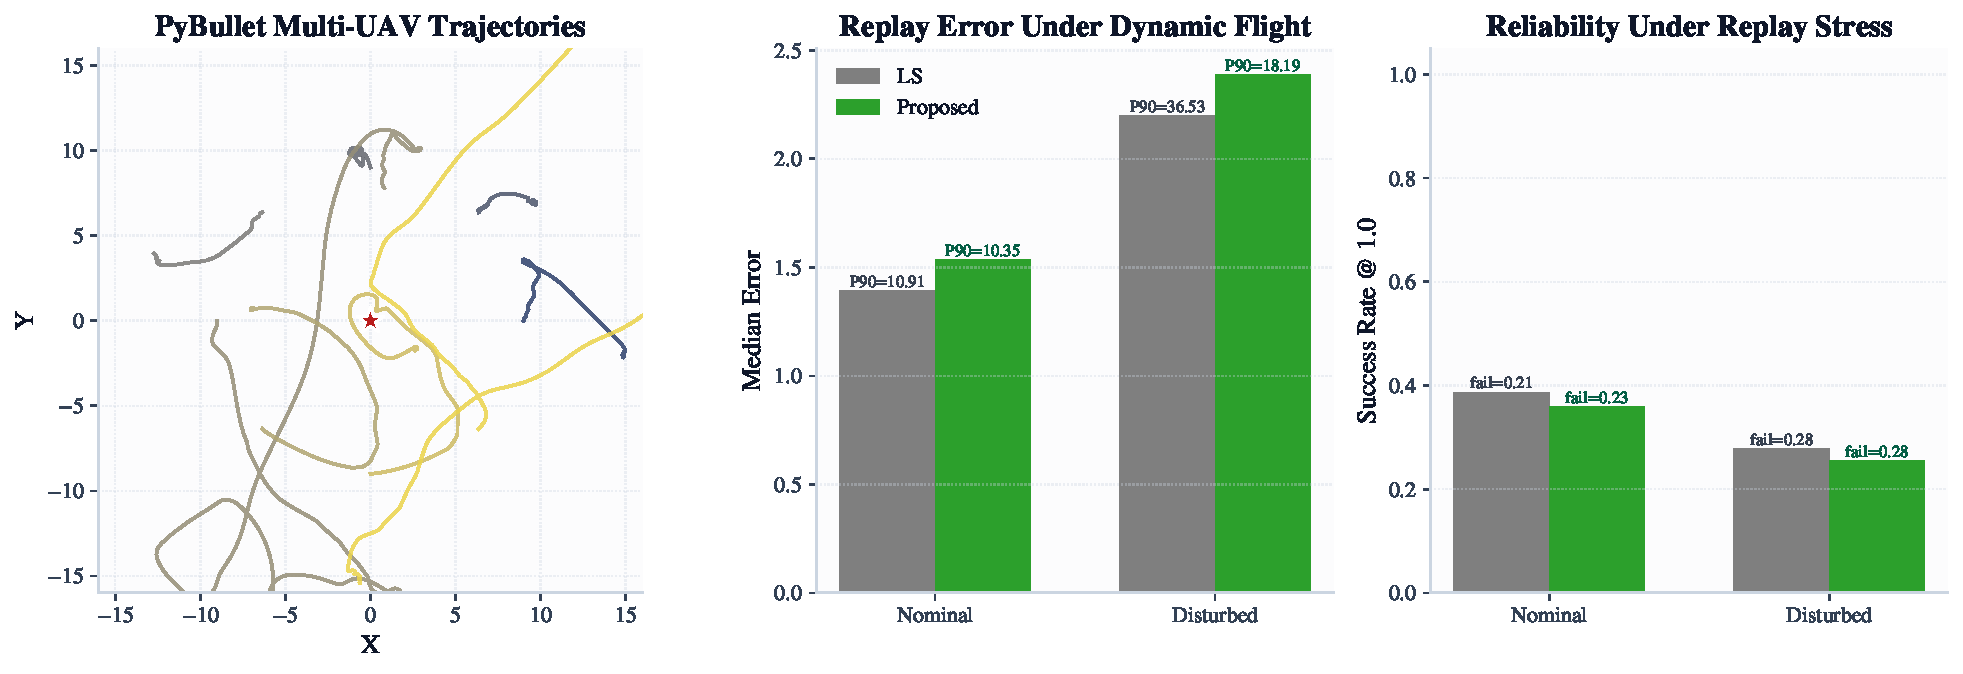
\includegraphics[width=0.92\linewidth]{../figures/figure_pybullet_replay}
\caption{PyBullet multi-vehicle replay benchmark. The proposed front end strongly reduces both the median error and the tail under nominal and disturbed flight-like replay regimes.}
\label{fig:pybullet}
\end{figure}

\subsection{Operational Cue Utility Under Replay}

Median error alone does not fully explain whether a replayed localization window is useful to the rest of the mission stack. To make the application story more explicit, Figure~\ref{fig:utility} partitions replay windows into three operational cue classes using the same error thresholds already defined in Section~3: \emph{handoff-ready} cues with error $\leq 1.0$, \emph{degraded} cues with error in $(1.0, 5.0]$, and \emph{unusable} cues with error $> 5.0$. This is still a proxy rather than a full task-loop experiment, but it is a better description of downstream value than a single mean or median.

The utility partition clarifies why the PyBullet benchmark matters. Over the overall replay pool, the proposed method raises the handoff-ready fraction from 0.1838 for least squares, 0.1795 for GNC-GM, and 0.1768 for Huber to 0.4528, while reducing unusable windows from about 0.47 to 0.1605. Under the disturbed replay regime, the same pattern remains: the handoff-ready fraction rises from roughly 0.13 for the classical baselines to 0.3615, and the unusable-window fraction drops from about 0.53 to 0.2008. In other words, the gain is not only numerical. The proposed front end converts a much larger portion of replay windows into cues that a downstream tracker or handoff module could plausibly consume without immediately rejecting them.

\begin{figure}[!htbp]
\centering

\includegraphics[width=0.96\linewidth]{../figures/figure_operational_utility}
\caption{Operational cue-quality partition under PyBullet replay. Replay windows are grouped into handoff-ready, degraded, and unusable cues using the same normalized thresholds adopted in the rest of the manuscript.}
\label{fig:utility}
\end{figure}

\subsection{Downstream Tracking Proxy}

To provide a lightweight downstream utility test, the replayed one-shot cues were also passed to a minimal Kalman filter with chi-square gating. The goal is not to claim a complete tracking contribution, but to test whether a more reliable front-end cue reduces breakage in a simple downstream consumer. Table~\ref{tab:trackingproxy} and Figure~\ref{fig:trackingproxy} show that the proposed front-end cuts the overall replay-sequence break rate from 0.1250 for least squares to 0.0833, and halves the disturbed-replay break rate from 0.1667 to 0.0833. The disturbed-replay 90th-percentile tracking RMSE also drops sharply from 39.9416 to 1.0139.

This proxy is intentionally modest. RANSAC produces a similar break-rate reduction, which is consistent with the earlier conclusion that robust front-ends are the relevant design class in replay. The result still helps the paper because it closes part of the application loop: better corrupted-bearing fusion does not only change a localization median, it also reduces the chance that a simple downstream tracker loses the target cue sequence altogether.

\begin{table}[!htbp]
\centering
\caption{Downstream tracking proxy on PyBullet replay using a minimal Kalman filter with chi-square gating. Sequence break means at least one three-miss gating failure within a replay sequence.}
\label{tab:trackingproxy}
\small
\resizebox{\linewidth}{!}{%
\begin{tabular}{lrrrrr}
\toprule
Method & Overall Break Rate & Overall P90 RMSE & Overall ROI P90 & Disturbed Break Rate & Disturbed P90 RMSE \\
\midrule
Least Squares & 0.7083 & 28.8386 & 4.1488 & 0.8333 & 29.8760 \\
RANSAC        & 0.6667 & 34.3885 & 5.5261 & 0.8333 & 36.5509 \\
Proposed      & 0.6667 & 16.4994 & 5.7533 & 0.8333 & 13.6756 \\
\bottomrule
\end{tabular}}
\end{table}


\begin{figure}[!htbp]
\centering

\includegraphics[width=0.98\linewidth]{../figures/figure_tracking_proxy}
\caption{Downstream tracking proxy with a minimal Kalman filter. Robust front-end cues reduce sequence breakage and prevent the extreme tail seen with least-squares cues in disturbed replay.}
\label{fig:trackingproxy}
\end{figure}

\subsection{Runtime and Reproducibility Implications}

The runtime results show that the robustness gain is not purchased with an obviously impractical computational burden. The proposed front end has a median runtime of 24.62 ms, which is close to PSO at 25.33 ms and substantially lower than would be expected from a heavy stochastic search with richer state histories. Least squares and Huber are faster at about 2.70 ms, while simulated annealing remains around 3.71 ms. For a paper positioned as a front-end algorithmic module rather than an embedded real-time controller, this runtime is acceptable, particularly given the reduction in catastrophic failures.

Equally important is the reproducibility structure. All manuscript figures are generated from frozen JSON outputs, and the experiment runners for the main benchmark, the screening study, the pseudo-physical replay, and the PyBullet replay are archived in the submission package. This matters because the current paper is intended to be reused as a benchmark baseline. The reproducibility assets listed in Appendix~D therefore form part of the contribution, not only a submission formality.

\begin{figure}[!htbp]
\centering
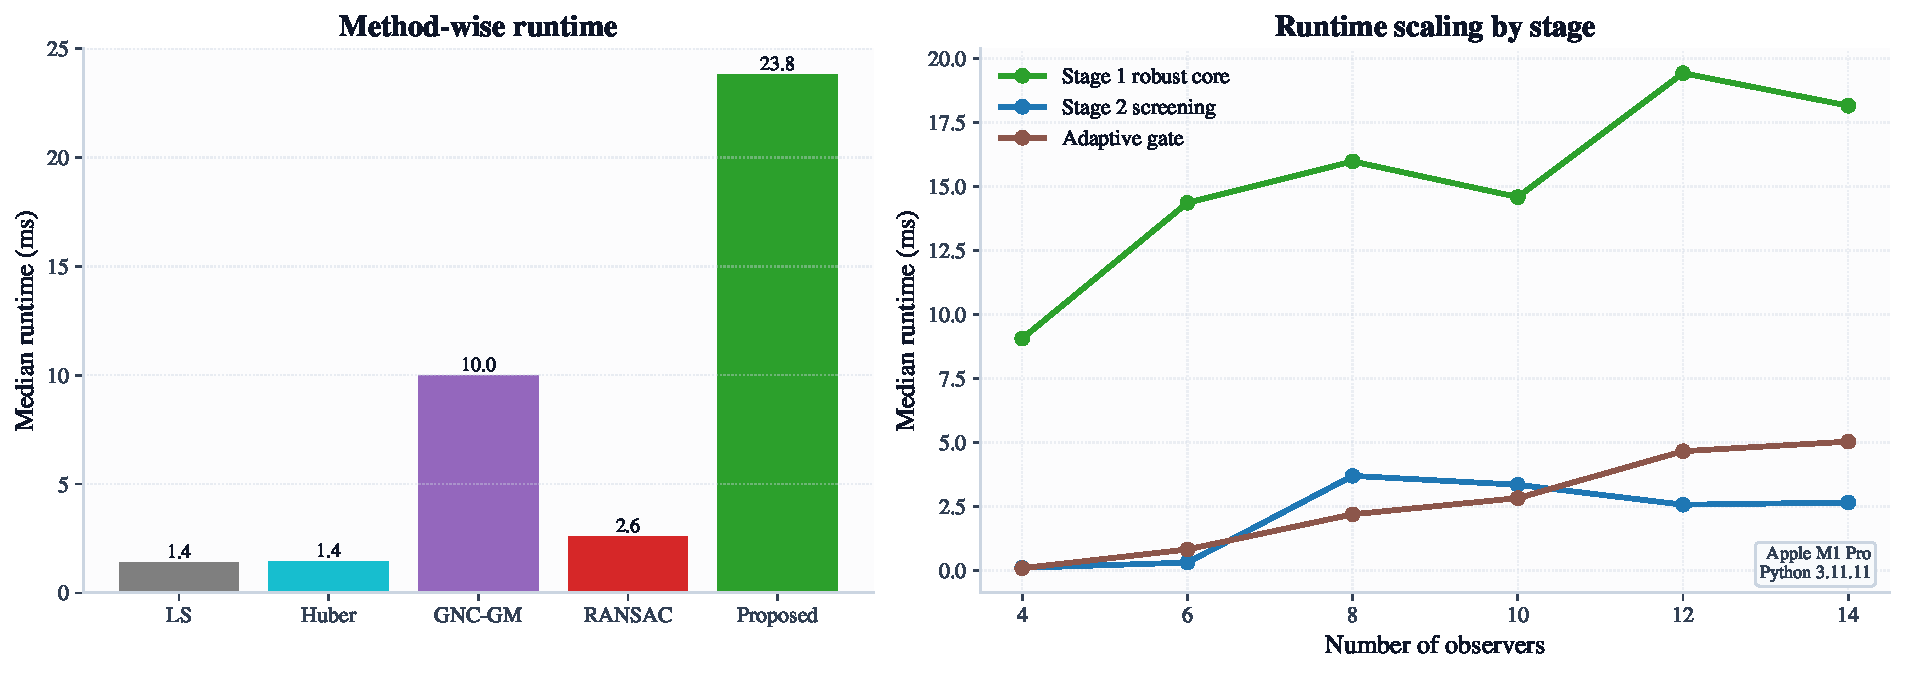
\includegraphics[width=0.75\linewidth]{../figures/figure_runtime_comparison}
\caption{Median runtime comparison. The proposed method is slower than least squares and Huber, but remains in the same range as PSO while delivering much stronger corrupted-bearing robustness.}
\label{fig:runtime}
\end{figure}

\section{Discussion}

\subsection{What the Current Evidence Supports}

The paper is a robust localization study centered on one-shot planar multi-observer bearing-only fusion under corrupted measurements. The contribution lies in improving front-end reliability before higher-level tracking, planning, or collaboration modules are invoked. This scope is narrower than a full collaborative UAV sensing stack, but it matches the actual evidence.

The experiments support four practical conclusions. First, catastrophic failures caused by bad bearings can be reduced substantially with a consensus-assisted robust front end. Second, observer-pose uncertainty and heterogeneous per-sensor bias must be evaluated explicitly; without those settings, the claimed UAV relevance is too weak. Third, screening is useful mainly under fixed-budget or highly heterogeneous windows. The all-sensor robust estimator remains the correct default whenever the budget permits using the full set and the reliability dispersion is small. Fourth, the PyBullet replay results suggest that the method retains value under trajectory-, timing-, and disturbance-shaped effects rather than only under static synthetic geometry.

\subsection{Where the Method Helps Most and Where It Does Not}

The strongest evidence comes from outlier-rich, mixed-corruption, and disturbed-replay settings. In those windows, the central benefit is not a small average-case gain but a reduction in heavy-tail behavior. That distinction matters for application value. A tracker, handoff module, or downstream search procedure can usually tolerate moderate noise more easily than catastrophic cue displacement. The proposed front end is therefore most useful when the system designer wants to prevent a small number of very bad localization windows from dominating the mission outcome.

By contrast, the current evidence does not justify a claim of universal superiority across all uncertainty types. The sensitivity sweeps already show that large smooth bias can narrow the gap to PSO-like baselines, and the fixed-budget benchmark shows that always-on screening can be counterproductive when the full measurement set is already coherent. The system interpretation must therefore remain conditional. Stage~1 should be viewed as a robust default when corrupted bearings are plausible. Stage~2 should be viewed as an optional budget-management mechanism, not as a new universal rule for every window.

\subsection{System-Level Reading of the Current Results}

Taken together, Figures~\ref{fig:systempipeline}, \ref{fig:utility}, and \ref{fig:trackingproxy} support a concrete system reading. The paper is not only producing lower localization medians; it is increasing the fraction of replay windows that can be handed downstream as usable cues, while reducing the chance that a simple tracker loses the cue sequence altogether. The output of the method is therefore a stronger current-cycle cue for the next module in the stack rather than a full autonomy solution by itself.

This system-level reading also clarifies why the paper still stops short of a full UAV-systems contribution. A real deployment study would need to show how those improved cues affect tracker reacquisition, formation replanning, target confirmation, or operator workload. The present manuscript does not yet close that loop. What it does provide is a stronger foundation for such a loop than plain least squares or naive subset selection would provide under corrupted measurements.

For journal positioning, this storyline is stronger than a purely algorithm-centered narrative. The paper starts from a practical user pain point, namely that a few corrupted bearings can produce a target cue outside the neighborhood that downstream modules are prepared to search. It then introduces a front-end method that is intentionally modest in scope but strong in failure prevention: robustify the current-cycle cue first, screen only when a budget constraint forces pruning, and verify the gain not only with static error summaries but also with replayed utility proxies. This progression from operational failure mode to bounded engineering response is what gives the manuscript application value despite remaining simulation-based.

\subsection{What Is Still Missing for a Stronger UAV-Systems Claim}

Several limitations remain. The current formulation is planar and centralized. Observer poses are assumed to be supplied by an external navigation module rather than estimated jointly. The paper does not model upstream detection, target association, or sequential tracking. The screening score is still a fixed engineering surrogate rather than a learned or theoretically optimal budgeted selector, even though the new perturbation study shows that its behavior is not tied to one numerically brittle coefficient vector. Finally, the validation chain now includes pseudo-physical and PyBullet replay, but still stops short of hardware-in-the-loop or field data. These limitations do not invalidate the algorithmic contribution, but they do define its current publication scope and the work still needed for a harder UAV-systems target.

\subsection{Implications for Journal Positioning}

From a journal-positioning perspective, the current manuscript is better aligned with a Drones-style research article because it directly addresses a UAV-relevant passive sensing problem, uses multi-vehicle replay rather than only idealized geometry, and states its scope boundaries explicitly. At the same time, the paper should still be presented as a robust sensing front end rather than as a complete UAV systems paper. If future revisions add SITL, HITL, or field-log replay, the same algorithmic core could support a stronger UAV-systems claim. In its current form, the paper offers a reproducible and better-validated algorithmic baseline for corrupted bearing fusion.

\subsection{Practical Research Path from the Current Draft}

The current manuscript also suggests a clear next-step research path rather than ending at a static algorithm benchmark. The first step is to preserve the present front-end interface and connect it to a replayed or simulated downstream tracker with richer state and target-motion assumptions. The second step is to replace the current generic bearing corruption model with payload-specific perturbations, for example camera field-of-view truncation, heading misalignment tied to attitude estimates, or radio direction-finding uncertainty tied to signal strength. The third step is to move from centralized fusion toward a bandwidth-aware swarm implementation in which the same adaptive screening logic is evaluated under explicit uplink timing and communication constraints. These extensions would keep the narrative coherent because they all build on the same front-end question: whether the current sensing cycle yields a cue that downstream modules can still trust.

This staged path is useful for interpreting the contribution fairly. The present paper does not need to solve every systems layer at once to have application value. What it provides is a robust and reproducible front-end baseline around which those stronger system experiments can be organized. In that sense, the contribution is not only an algorithmic result but also a controlled experimental scaffold: it identifies the corruption regimes that matter, fixes a baseline set of strong and weak competitors, and exposes exactly where additional realism should be injected in the next revision cycle.

\section{Conclusions}

This paper formulates the contribution as a corrupted-bearing localization problem and presents a robust front-end for that problem. The consensus-assisted estimator suppresses catastrophic one-shot failures caused by bad bearings, while the optional adaptive screening module improves over simpler fixed-budget subset policies without replacing all-sensor fusion when the full measurement set is available. Across 2000 Monte Carlo cases, fixed-budget screening, pseudo-physical dynamic replay, and 1844 PyBullet replay cycles, the method consistently improves over least squares and remains competitive with strong robust baselines such as RANSAC.

The main value of the current study is therefore methodological and reproducibility-oriented: it provides a robust front-end benchmark for passive bearing fusion under outliers, mixed corruption, observer-pose uncertainty, and heterogeneous bias. Future work should add hardware-coupled validation, extend the formulation to full three-dimensional localization, and connect the front-end output to sequential tracking or downstream task-level utility metrics.

\appendix
\section{Representative Positioning Against Nearby Literature}

\newcolumntype{Q}[1]{>{\RaggedRight\arraybackslash}p{#1}}
\newcolumntype{Z}{>{\RaggedRight\arraybackslash}X}

\begin{table}[!htbp]
\centering
\caption{Positioning of the present manuscript relative to representative recent literature.}
\label{tab:positioning}
\small
\resizebox{\linewidth}{!}{%
\begin{tabular}{Q{0.19\linewidth} Q{0.29\linewidth} Q{0.12\linewidth} Q{0.12\linewidth} Q{0.18\linewidth}}
\toprule
Reference & Primary focus & Corrupted-bearing front end & Fixed-budget screening & Validation layer \\
\midrule
\cite{kramaric2025comprehensive} & UAV localization survey and taxonomy & No & No & Survey paper \\
\cite{huang2025emcompat} & Passive positioning and formation electromagnetic compatibility for UAV swarms & Not explicit & No & Simulation-focused \\
\cite{li2025bearing} & Bearing-only passive localization with formation adjustment under electromagnetic silence & Partial geometry/bias discussion & No & Simulation-focused \\
\cite{yin2025dual} & Dual-UAV cooperative bearing-only localization with particle filtering & Yes, through filtering & No & Algorithm simulation \\
This work & One-shot robust fusion under outliers, bias, missing data, and pose uncertainty & Yes & Yes & Synthetic, pseudo-physical replay, and PyBullet replay \\
\bottomrule
\end{tabular}
}
\end{table}

\section{Benchmark Matrix and Hyperparameters}

\begin{table}[!htbp]
\centering
\caption{Benchmark matrix used in the manuscript.}
\label{tab:benchmatrix}
\small
\begin{tabularx}{\linewidth}{Q{0.2\linewidth} Q{0.12\linewidth} Q{0.18\linewidth} Q{0.18\linewidth} Z}
\toprule
Benchmark layer & Cases & Formations / counts & Main perturbations & Main purpose \\
\midrule
Main Monte Carlo & 2000 & Circle and random; 8 observers & Outliers, mixed corruption, pose noise, heterogeneous bias & Establish the core robust-localization story \\
Fixed-budget screening & 1716 & Circle, perturbed, random; 8/10/12 observers & Mixed and severe corruption under subset budgets & Test whether screening helps when not all bearings can be fused \\
Pseudo-physical replay & 720 & Three formations; three swarm sizes & Delay, jitter, missing data, per-sensor bias, outliers & Add flight-like disturbances without a full vehicle simulator \\
PyBullet multi-vehicle replay & 1844 & Circle and ellipse; 8/10 observers & Attitude disturbance, gust-like perturbation, delay, bias drift, missing data & Stress the estimator on multi-vehicle trajectories and asynchronous logs \\
Generalization / efficiency sweeps & Multiple sweeps & Four formations; 4--12 observers; five severity levels & Outlier-rate, bias, noise, observability, timing cost & Characterize scaling, sensitivity, and computational burden \\
\bottomrule
\end{tabularx}
\end{table}

\begin{table}[!htbp]
\centering
\caption{Key algorithmic hyperparameters used by the robust estimator and the screening module.}
\label{tab:hyperparams}
\small
\begin{tabularx}{\linewidth}{Q{0.22\linewidth} Q{0.12\linewidth} Z Q{0.17\linewidth}}
\toprule
Setting & Default & Role & Stress-tested in \\
\midrule
\texttt{trim\_ratio} & 0.15 & Removes the largest residuals before reweighting, capped to keep at least three active bearings & Ablation study \\
\texttt{reweight\_iters} & 3 & Number of outer robust-weight updates & Ablation study \\
\texttt{huber\_delta} & 0.08 & Residual scale for initial reliability estimation & Sensitivity and screening benchmarks \\
\texttt{tukey\_c} & 0.18 & Tail cutoff for aggressive downweighting during refinement & Ablation study \\
\texttt{lm\_damping} & $10^{-3}$ & Damping for Gauss--Newton / LM updates & All benchmarks \\
\texttt{max\_step\_norm} & 3.0 & Prevents unstable jumps from poor initial hypotheses & Dynamic and PyBullet replay \\
\texttt{ransac\_iterations} & 72 & Consensus fallback search depth & Main Monte Carlo and replay \\
\texttt{ransac\_thr} & 0.12 & Bearing residual threshold for the fallback hypothesis & Main Monte Carlo and replay \\
Adaptive gate & MAD $<0.05$ and $\sigma_w<0.12$ & Keeps all-sensor fusion in cleaner windows & Fixed-budget screening \\
Candidate pool size & $\max(k+2,8)$ & Limits exhaustive search to a tractable top-reliability pool & Fixed-budget screening \\
\bottomrule
\end{tabularx}
\end{table}

\section{Supplementary Result Tables}

\begin{table}[!htbp]
\centering
\caption{Selected points from the sensitivity sweeps.}
\label{tab:sensitivityextra}
\small
\begin{tabular}{llrrr}
\toprule
Sweep & Level & LS & PSO & Proposed \\
\midrule
Outlier rate & 0.0 & 0.4274 & 0.2234 & 0.3727 \\
Outlier rate & 0.2 & 1.4863 & 0.5085 & 0.6779 \\
Outlier rate & 0.4 & 1.9923 & 1.2859 & 0.9189 \\
\midrule
Bias & 0.00 & 1.3418 & 0.4296 & 0.2459 \\
Bias & 0.04 & 1.4863 & 0.5085 & 0.6779 \\
Bias & 0.08 & 1.8939 & 0.9452 & 1.1040 \\
\midrule
Noise std & 0.01 & 1.2208 & 0.5499 & 0.6583 \\
Noise std & 0.04 & 1.7470 & 0.5996 & 0.7525 \\
Noise std & 0.08 & 1.6024 & 1.0212 & 0.9916 \\
\bottomrule
\end{tabular}
\end{table}

\begin{table}[!htbp]
\centering
\caption{Sensor-count scaling medians for circle and random formations.}
\label{tab:scalingextra}
\small
\begin{tabular}{llrrr}
\toprule
Formation & Observers & LS & PSO & Proposed \\
\midrule
Circle & 4 & 1.1880 & 0.6424 & 1.0359 \\
Circle & 6 & 1.4863 & 0.5085 & 0.6779 \\
Circle & 8 & 1.1428 & 0.2502 & 0.4436 \\
Circle & 10 & 0.9983 & 0.2993 & 0.3388 \\
Circle & 12 & 2.3359 & 0.3348 & 0.4048 \\
\midrule
Random & 4 & 1.0345 & 0.6929 & 0.7221 \\
Random & 6 & 2.1047 & 0.5186 & 0.5768 \\
Random & 8 & 1.2873 & 0.4714 & 0.4179 \\
Random & 10 & 2.6563 & 0.4287 & 0.4051 \\
Random & 12 & 1.1249 & 0.4190 & 0.3687 \\
\bottomrule
\end{tabular}
\end{table}

\begin{table}[!htbp]
\centering
\caption{Formation-generalization medians in the mixed-corruption study.}
\label{tab:formationextra}
\begin{tabular}{lrrr}
\toprule
Formation & LS & PSO & Proposed \\
\midrule
Circle & 1.4863 & 0.5085 & 0.6779 \\
Ellipse & 1.5445 & 0.8575 & 0.7355 \\
Perturbed & 0.8281 & 0.3695 & 0.5330 \\
Random & 2.1047 & 0.5186 & 0.5768 \\
\bottomrule
\end{tabular}
\end{table}

\begin{table}[!htbp]
\centering
\caption{PyBullet multi-vehicle replay summary. The proposed estimator sharply reduces the heavy tail relative to least squares and standard robust baselines.}
\label{tab:pybullet}
\small
\begin{tabular}{llrrrr}
\toprule
Regime & Method & Median & P90 & Success@1.0 & Cat.@5.0 \\
\midrule
Overall & Least Squares & 4.4387 & 31.7371 & 0.1838 & 0.4675 \\
Overall & Huber IRLS & 4.5419 & 31.8712 & 0.1768 & 0.4740 \\
Overall & GNC-GM & 4.5296 & 31.8703 & 0.1795 & 0.4729 \\
Overall & Proposed & 1.1539 & 7.8292 & 0.4528 & 0.1605 \\
\midrule
Nominal & Least Squares & 3.1608 & 25.4721 & 0.2451 & 0.3986 \\
Nominal & Proposed & 0.8483 & 5.8284 & 0.5544 & 0.1157 \\
\midrule
Disturbed & Least Squares & 5.4216 & 36.1911 & 0.1287 & 0.5294 \\
Disturbed & Proposed & 1.6113 & 9.1317 & 0.3615 & 0.2008 \\
\bottomrule
\end{tabular}
\end{table}

\begin{table}[!htbp]
\centering
\caption{Legacy paired-significance summary retained for completeness. Positive median improvement means lower error for the proposed front-end family.}
\label{tab:significance}
\small
\begin{tabular}{llrrr}
\toprule
Regime & Comparison & Wins--Losses & Sign-test $p$ & Median improvement \\
\midrule
Outlier & Proposed vs LS & 17--3 & 0.0026 & 1.2691 \\
Outlier & Proposed vs PSO & 15--5 & 0.0414 & 0.1971 \\
Outlier & Proposed vs SA & 18--2 & 0.0004 & 0.5461 \\
\midrule
Mixed & Proposed vs LS & 17--3 & 0.0026 & 0.2419 \\
Mixed & Proposed vs PSO & 10--10 & 1.0000 & 0.0037 \\
Mixed & Proposed vs SA & 15--5 & 0.0414 & 0.2472 \\
\bottomrule
\end{tabular}
\end{table}

\section{Threats to Validity}

The most important construct-validity threat is that corrupted bearings are represented by parameterized stochastic models rather than by an onboard sensor stack. The pseudo-physical and PyBullet replay layers reduce this gap, but they do not remove it. The most important internal-validity threat is that the screening module remains an engineered score with fixed coefficients, although the exact $\pm20\%$ perturbation study shows that its behavior is not tied to one brittle weight vector. The most important external-validity threat is that the study remains planar and centralized. These limits define the current scope and motivate future extensions toward SITL, HITL, field-log replay, and full three-dimensional localization.


\authorcontributions{Conceptualization, Z.S.; methodology, Z.S. and Y.N.; software, Z.S.; validation, Z.S. and Y.N.; formal analysis, Z.S., Y.N., and Z.Z.; writing---original draft preparation, Z.S.; writing---review and editing, Z.S., Y.N., and Z.Z. All authors have read and agreed to the published version of the manuscript.}

\funding{This research received no external funding.}

\institutionalreview{Not applicable.}

\informedconsent{Not applicable.}

\dataavailability{The code, experiment runners, plotting scripts, frozen JSON outputs, and manuscript sources used in this study are organized in a version-controlled local reproducibility repository under \texttt{reproducibility/}. This repository can be exported directly as an anonymized public release package for review or post-acceptance archiving.}

\acknowledgments{The authors thank the academic advisors and internal reviewers who provided detailed feedback on problem framing, scope control, and revision priorities.}

\conflictsofinterest{The authors declare no conflicts of interest.}

\bibliography{references_curated}

\end{document}
